% Earned Autonomy for AI Agents -- LaTeX version (PLAN_SUITE T30).
% body.tex, abstract.tex, refs.bib and tables/*.tex are generated by outils/construire_latex.py; do not edit them.
\documentclass[11pt,letterpaper]{article}
\usepackage[T1]{fontenc}
\usepackage[utf8]{inputenc}
\usepackage{lmodern}
\usepackage[margin=1in]{geometry}
\usepackage{amsmath,amssymb}
\usepackage{graphicx}
\usepackage{booktabs,longtable,array,calc}
\usepackage{caption}
\usepackage{xcolor}
\usepackage{microtype}
\usepackage{xurl}
\usepackage[hidelinks]{hyperref}
\usepackage{newunicodechar}


% Unicode characters used in the draft (pdfLaTeX, as on arXiv)
\newunicodechar{τ}{\ensuremath{\tau}}
\newunicodechar{ρ}{\ensuremath{\rho}}
\newunicodechar{α}{\ensuremath{\alpha}}
\newunicodechar{×}{\ensuremath{\times}}
\newunicodechar{≥}{\ensuremath{\geq}}
\newunicodechar{≤}{\ensuremath{\leq}}
\newunicodechar{−}{\ensuremath{-}}
\newunicodechar{≈}{\ensuremath{\approx}}
\newunicodechar{÷}{\ensuremath{\div}}
\newunicodechar{→}{\ensuremath{\to}}
\newunicodechar{½}{\ensuremath{\tfrac12}}
\newunicodechar{¼}{\ensuremath{\tfrac14}}
\newunicodechar{²}{\textsuperscript{2}}
\newunicodechar{≠}{\ensuremath{\neq}}
\newunicodechar{∞}{\ensuremath{\infty}}
\newunicodechar{·}{\ensuremath{\cdot}}
\newunicodechar{√}{\ensuremath{\surd}}
\newunicodechar{∈}{\ensuremath{\in}}
\newunicodechar{β}{\ensuremath{\beta}}
\newunicodechar{ℓ}{\ensuremath{\ell}}
\newunicodechar{⌈}{\ensuremath{\lceil}}
\newunicodechar{⌉}{\ensuremath{\rceil}}
\newunicodechar{…}{\ldots}

% Commands emitted by pandoc
\newcounter{none}
\providecommand{\pandocbounded}[1]{#1}
\providecommand{\tightlist}{\setlength{\itemsep}{0pt}\setlength{\parskip}{0pt}}
\makeatletter
\def\maxwidth{\ifdim\Gin@nat@width>\linewidth\linewidth\else\Gin@nat@width\fi}
\makeatother
\setcounter{secnumdepth}{0}

\title{Earned Autonomy for AI Agents: A Pre-registered Error-Budget Test of Per-Action-Type Delegation}
\author{Otsoa Dubief\\ \small Independent researcher, \texttt{otsoa.dubief@gmail.com}, ORCID 0009-0002-7322-7575\\ \small Preregistration: \url{https://osf.io/vycge/} (frozen at git tag \texttt{gel-2026-11-09})\\ \small Priority record: \url{https://osf.io/7ju3c/}\\[4pt] \footnotesize The agents evaluated, the alert reviewers and the writing assistant are Claude models;\\ \footnotesize API costs were covered by Anthropic startup credits (see Declarations).}
\date{Draft, 18 November 2026}

\begin{document}
\maketitle

\begin{abstract}
Which actions may an AI agent take without human sign-off? We propose an open rule: an agent earns autonomy on one action type after N consecutive verified successes and loses it at the first confirmed error; N is derived from an error budget fixed in advance per stakes level by adapting the unrestricted AOQL of continuous sampling plans, with a conditional bound on the extra errors delegation lets through. We test it in a pre-registered replay: three Claude 5.5 models on four public benchmarks (τ-bench airline, retail and banking; WorkBench), 14,266 episodes played (13,623 analysed), writes checked by exact comparison (98.7\% coverage) and alerts reviewed on blind sheets by separate Claude instances. No configuration reached the pre-registered level of evidence required for delegation (verdict R4). Only one of twelve configurations had enough volume to be judged; its error rate, 8.6\% (lower bound 4.1\%), is established above the 0.76\% threshold. Of its 79 errors, 48 are one plot end-date discrepancy reviewers decided both ways; lifting it throughout leaves 31, established by two errors, and lifting also four one-day window shifts would not. The other eleven had too little effective volume to conclude either way. Descriptively (no multiplicity correction), 20 of 40 model--environment--type combinations have an error rate established above their threshold (11 of them on banking); 13 show no observed error but too little volume. The rule was not refuted, but it was hardly put to the test, and its usefulness could not be judged. These rates count action errors confirmed by review against a single expected path per task; in a blind sample reviewed by the author, 3 of 10 confirmed alerts were lifted, too few to rule out false-alert shares that would overturn the judged excess. As the plan stated in advance, earning autonomy under such budgets takes far more verified actions than these benchmarks provide at our volumes.

\end{abstract}

\subsection{1 Introduction}\label{introduction}

An agent that books flights, refunds orders or files calendar entries takes dozens of actions per task. Most are reads; some change the state of the world. The question every deployment faces is: \emph{which of these actions can the agent take alone, and on what evidence?} Current practice answers with fixed allow-lists, with a risk triage that ignores the agent's record, or with trust that grows without a stated criterion. None ties the decision to the agent's observed record on that kind of action, and none says how many errors the arrangement lets through.

We study an alternative from industrial quality control. In a continuous sampling plan (Dodge, 1943, p.~265), every unit is inspected until i consecutive units conform; inspection then drops to a fraction and returns to 100 \% at the first defect. Read in reverse for agents: validate every action of a type until the agent has N consecutive verified successes on it, then let it act alone on that type, and withdraw autonomy at the first error. Without any assumption of statistical control, such a plan bounds outgoing quality (Lieberman, 1953, pp.~480-482; Derman, Johns and Lieberman, 1959, pp.~1176-1177), and a cycle argument gives a conditional bound on the extra errors that delegation lets through (detected errors, immediate detection, a write mix close to the expected one; Section 3).

\textbf{Contributions.} (1) A complete, open rule for earned autonomy \emph{per action type}, whose run length N is derived from an error budget fixed in advance, with a conditional bound on the extra errors (Section 3). (2) A measurement of the \emph{delegation gap}: for each model, environment and action type observed, the confirmed error rate against the bar the budget requires, with its interval; half of these types remain undetermined (Section 6.4). (3) A pre-registered protocol, in which, at our volumes, only types with enough effective writes could decide the label; one did (Section 6.2). The plan stated in advance that at these volumes no type could be certified below its bar and that the high-stakes run lengths exceed the data: plan, rule, code, seeds and labels were registered on OSF on 10 November 2026 at 05:00 UTC, before wave 1 started at 05:19 UTC; alerts are reviewed on blind sheets by separate Claude instances, and a blind sample by the author; the calibration/confirmation split is drawn from a public randomness beacon after the confirmed verdicts are frozen.

\textbf{Results in brief.} None of the twelve configurations reached the pre-registered level of evidence required for delegation (label R4). Only Haiku on WorkBench had enough volume to be judged: its reversible writes have a confirmed action-error rate of 8.6 \% on the calibration half against a 0.76 \% bar (48 of its 79 errors are one plot end-date discrepancy that the reviewers decided both ways; lifting it throughout leaves 3.4 \%, established by a two-error margin; Section 6.7) (errors against a single expected path per task; Haiku's task success on WorkBench is 95 \% to 97 \% per half, and 64 \% of its episodes with a confirmed error over the whole reserve are successful tasks). Descriptively, of 40 observed model--environment--type combinations, 20 have an error rate established above their bar (11 of them on banking, where agent and setup errors cannot be separated), 13 show no observed error but too little volume, and none could be shown below its bar at these volumes. The safety criterion was not refuted, but with almost no power; utility could not be judged.

\subsection{2 Related work}\label{related-work}

\emph{Quality control.} Continuous sampling plans (Dodge, 1943), their tolerant (Dodge and Torrey, 1951, as reported by Hryniewicz, 2011), multi-level (Lieberman and Solomon, 1955) and tightened (Derman, Littauer and Solomon, 1957) variants, and the unrestricted AOQL (Lieberman, 1953; Derman, Johns and Lieberman, 1959) provide our template; Wald and Wolfowitz (1945, p.~47) had noted that Dodge's AOQL formulas need statistical control, and Hillier (1964) proposed a limit on extra defectives after a jump. Our bound adapts the UAOQL cycle argument to a check that follows execution; we do not claim it as new. \emph{Levels of autonomy.} Parasuraman, Sheridan and Wickens (2000) and Feng, McDonald and Zhang (2025) define levels without a statistical mechanism for moving between them; Weber and Taneja (2026) promote per skill on windows of N outputs and a correction-rate threshold, with no budget-derived N or bound. \emph{Error budgets.} CASE (Telukunta, Lilis and Baron, 2026) makes autonomy a non-decreasing function of the remaining error budget (Eq. 7, p.~10) and already speaks of autonomy ``earned against a measured error budget'' (p.~11); the function is unspecified and untested. \emph{Earned authority.} Zhang and Zhang (2026) formalise authority that falls freely, rises only under an abstract evidence relation and stays below a user-fixed ceiling; we instantiate that relation and put it to a pre-registered test, which had little power (Section 6.3). \emph{Statistics of evaluations.} We follow Miller (2024): the task is the independent unit, rules are compared on the same traces, and intervals come from a task-level jackknife-t; simultaneous inference uses max-T (Westfall and Young, 1993). The extended version of this paper (\texttt{article/\allowbreak{}brouillon.\allowbreak{}md} in the code archive; see Appendix F) gives the full related work, including selective classification, AI control and agent benchmarks.

\subsection{3 The rule}\label{the-rule}

\textbf{Action types and caps.} A frozen table maps each benchmark tool to a type, a stakes level and reversibility: low (read, reversible write ECR, internal message MSG), medium (durable write DUR, execution), high (external output, money ARG, guardrail or rights GAR, illegible effect ILL). Evidence stays within its type. Reads are autonomous and uncounted; the budget is counted per write. Some actions are always validated (caps): guardrails and rights, consent, secrets, money above a per-environment amount, a first message to an unknown recipient. The idea of a ceiling that evidence cannot lift follows Zhang and Zhang (2026).

\textbf{Tiers and B-all.} Tier 1: \emph{ask before}; tier 2: \emph{act then notify} (reversible types); tier 3: \emph{act alone}. Under the main rule, \textbf{B-all} (named B-tout in the frozen plan), a type reaches tier 3 after N consecutive verified successes; any error resets the counter; an error at tier 3 withdraws autonomy (to tier 1 with a trial at medium and high stakes); a model change resets the counter. Below tier 3, tier 2 follows a Wald (1945) sequential score. An automated check judges each write; an alert counts as an error only after confirmation.

\textbf{From a budget to N.} The author fixed, blind and in advance, the extra errors he would accept relative to ``validate everything'': 0.5, 0.05 and 0.005 per 100 writes at low, medium and high stakes. The budget becomes a per-type \emph{bar}, bar = B/(0.95 × 100 × q), where q is the expected share of the level's writes, and N = ⌈1/(d × bar)⌉ − 1 with d = 0.95 the assumed detection share. N ranges from 12 to 138 at low stakes, 204 to 733 at medium and 2,582 to 12,653 at high stakes (Appendix B, Table 1).

\textbf{Conditional guarantee.} Each autonomy period follows at least N verified successes and ends at the first detected error. Counting in cycles, the expected number of errors executed at tier 3 per write of the type is at most 1/(1 + N d), whatever the error sequence; with immediate and complete detection, at most one executed error per N + 1 writes. At a level, the extra errors stay below 0.95 × budget × s/q, where s is the real share of the level's writes. The bound assumes immediate detection of the errors the check sees and misses that are random rather than targeted; it is a long-run bound when d \textless{} 1 (Section B.3.4).

\subsection{4 Setup}\label{setup}

\textbf{Benchmarks and models.} Four public environments: τ-bench 2.0 airline, retail and banking (Yao et al., 2024; Barres et al., 2025; Shi et al., 2026), and WorkBench (Styles et al., 2024), graded without any LLM judge; 20 \% of tasks served for a pilot and never enter the verdict. Agents: Claude Haiku, Sonnet and Opus 5.5 with default settings; the τ-bench simulated user is Haiku 5.5. A \emph{configuration} is one model in one environment (12). 14,266 episodes were planned (Haiku 50 passes on airline and retail, 10 on banking, 5 on WorkBench; Sonnet and Opus 10, 10, 3 and 1).

\textbf{Instrument.} Every write made with a tool of the frozen table is judged by exact comparison with the task's expected actions. Every alert (a write marked wrong, duplicate or refused) is reviewed by fresh Claude instances on blind sheets and can be lifted only for one of four pre-written reasons with proof: defective task, rephrasing of a free-text field, another path allowed by the policy, or a defect of our code. In each wave the author blind-reviews 15 alerts; at least 13 agreements keep the review.

\textbf{Halves, draw and replay.} The reserve is split by task into a \emph{calibration} half, which measures each configuration's error rate by type and decides delegability, and a \emph{confirmation} half, where the frozen rule is replayed once. The split was drawn from a NIST beacon pulse after the confirmed verdicts were frozen and registered (OSF cusv6). The rule and its comparators (``validate everything'', a fixed list, a risk triage) are replayed offline on the recorded episodes with a simulated validator that misses 5 \% of errors, 2,000 replays per configuration (Appendix B).

\subsection{5 Pre-registered analysis}\label{pre-registered-analysis}

\textbf{Labels.} Point 0 checks the instrument (coverage ≥ 0.95, blind review kept). H1 (safety, eliminatory): B-all has no established budget excess (max-T) in any of 180 cells (12 configurations and 48 model-change sequences × 3 stakes levels); a failure gives R1. A configuration is \emph{delegable} if at least one type has a median calibration rate at most its bar; a type is \emph{judgeable} if zero errors would bring it under its bar (\(n_{\mathrm{eff}} \times \mathrm{bar}\) at least about ln 2, 0.6905 at the WorkBench low-stakes bar), where \(n_{\mathrm{eff}} = n/(1 + (\bar m - 1)\hat\rho)\) is the effective number of the type's \(n\) writes under the estimated within-task correlation \(\hat\rho\) (\(\bar m\): writes per task, weighted). A rate is \emph{established above} its bar when its lower bound lies above it. If no configuration is delegable, the label is R4 when at least one type is judgeable and every configuration with a judgeable type has one whose one-sided 95 \% Clopper--Pearson lower bound at ρ = 1 lies above its bar; otherwise ``insufficient evidence''. R4's registered name is ``nothing to delegate: unreliability established''; we keep the label, not the name, as a description, since what is established concerns one action type in one configuration (Section 6.2). H2 (utility) compares loads over delegable configurations; it is not judged under R4. Order: R5, R1, insufficient evidence, R4, R2, confirmed.

\textbf{What the labels can mean.} With immediate detection the bound holds for any sequence, so H1 can hardly fail through the data; R1 could mean a mix gap (s above about 1.05 × q), not that agents are unreliable. The part that can really fail is H2, together with the delegation gap. Lower bounds are per type, without multiplicity correction, under the effective-size approximation (Appendix C).

\subsection{6 Results}\label{results}

\textbf{Collection and instrument (6.1).} All 14,266 planned episodes were played; 91 were excluded, all for an empty agent message that τ-bench records as an infrastructure error (77 Haiku on banking); 13,623 are analysed after exclusions and removal of 12 defective tasks. These exclusions remove agent failures and favour delegation. Instrument coverage was 98.7 \% (banking 92.5 \% to 93.0 \%). 2,761 alerts were reviewed: 1,991 confirmed and 770 lifted. The author's blind review agreed 13 of 15 times in each wave, exactly the threshold; three of the four disagreements lifted a confirmed alert, and the pre-registered re-review of all lifted high-stakes alerts was not triggered. API spend was 837.19 USD, above the pre-registered estimate (517 to 674 USD). Appendix C gives the full account.

\textbf{Label (6.2).} No configuration reached the pre-registered level of evidence required for delegation (label R4). Only one of twelve had enough volume to be judged (Haiku on WorkBench, reversible writes): its confirmed error rate, 8.6 \% (914 writes, 79 errors; lower bound 4.1 \% at ρ = 1), is established above its 0.76 \% bar. The other eleven have no judgeable type. Judgeability is narrow and rests on the estimated correlation: \(n_{\mathrm{eff}} \times \mathrm{bar} = 0.740\) against 0.6905 at \ensuremath{\hat{\rho}} = 0.819 (\(n_{\mathrm{eff}} = 97.7\)); at ρ = 1 (\(n_{\mathrm{eff}} = 81.6\), product 0.618) the type would not be judgeable, and above \ensuremath{\hat{\rho}} = 0.885 the label would become ``insufficient evidence'' (a post hoc computation; Appendix D gives an approximate bootstrap interval for \ensuremath{\hat{\rho}}, with a simpler estimator than the engine's). The excess is established at ρ = 1; the judgeability that makes it count is not. Raw verdicts and the role swap also give R4, but they sit at the edge of the same threshold.

\textbf{Safety (6.3).} Point 1 is held in the sense of ``not refuted'', with almost no power: no established excess, but an excess would have needed an estimate more than seven standard errors above the budget (c* = 7.0), and no cell is demonstrated below budget. Of 180 cells, 51 were judged (all at low stakes), 108 held without being put to the test and 21 were without object. Central estimates stay at most 0.38 times the budget (Figure 1). In 24 judged cells (WorkBench and banking) s/q exceeds 1/0.95, so the construction bound alone does not guarantee the budget there.

\begin{figure}
\centering
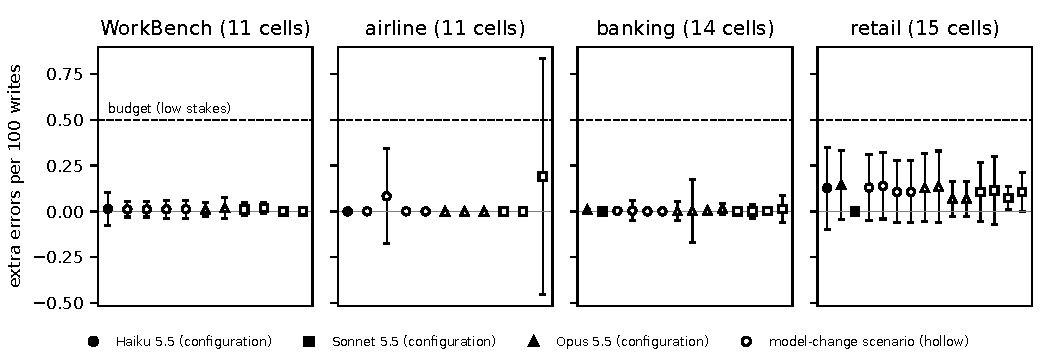
\includegraphics[width=1\linewidth,height=\textheight,keepaspectratio,alt={Extra errors per 100 writes against the budget, B-all, the 51 judged cells (main analysis). Filled markers: configurations; hollow: model-change scenarios. Bars: nominal 95 \% intervals, read descriptively. Dashed line: low-stakes budget.}]{../figures/fig1_budget.pdf}
\caption{Extra errors per 100 writes against the budget, B-all, the 51 judged cells (main analysis). Filled markers: configurations; hollow: model-change scenarios. Bars: nominal 95 \% intervals, read descriptively. Dashed line: low-stakes budget.}\label{fig:budget}
\end{figure}

\textbf{Delegation gap (6.4).} Descriptively and without multiplicity correction, 20 of the 40 model--environment--type combinations are above their bar at ρ = 1, 20 undetermined, none below; at these volumes the table could only return ``above'' or ``undetermined''. Of the 20, 11 are on banking, 6 are money-moving writes on airline and retail, and 3 are reversible writes on WorkBench. The 13 types without observed errors have 3 to 122 writes. On WorkBench, reversible writes err 5.5 \% to 8.6 \% against a 0.76 \% bar (lower bound ÷ bar 2.7 to 5.5), with similar rates on the confirmation half (5.9 \% to 11.0 \%). Money-moving writes on airline and retail err 6.5 \% to 13.3 \% on the calibration half against bars near 0.008 \% (Figure 2), but 1.2 \% to 7.7 \% on the confirmation half (3.8 \% to 8.0 \% on the whole reserve): the two halves differ by up to a factor of five, and the intervals are wide (upper bounds 20 \% to 51 \%). At such bars a single error in 500 writes already gives a ratio of about 20: the high-stakes ratios mostly measure the budget chosen. Banking rates are higher (28 \% to 56 \% for money-moving and medium-stakes writes), but banking is where attribution to the agent is weakest (coverage 0.925, unmapped tools, a knowledge base not shown to reviewers, high stakes carried by the simulated client, 89 of 91 exclusions). On the whole reserve (descriptive), three configurations would have had a delegable type, all with zero observed errors (Appendix C, Table 6 bis).

\begin{figure}
\centering
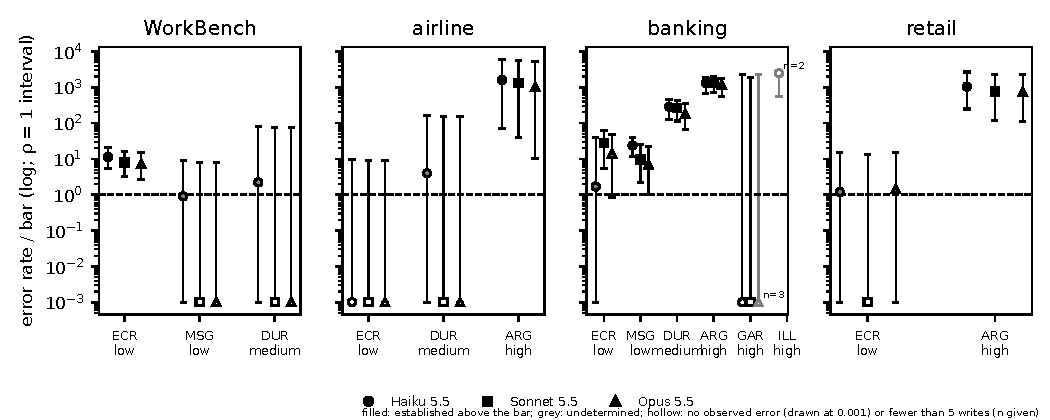
\includegraphics[width=1\linewidth,height=\textheight,keepaspectratio,alt={Delegation gap: confirmed error rate divided by the bar, with the ρ = 1 interval, log scale, calibration half. Filled: established above the bar; grey: undetermined; hollow: no observed error (drawn at 0.001) or fewer than 5 writes (n given). Dashed line: the bar.}]{../figures/fig2_gap.pdf}
\caption{Delegation gap: confirmed error rate divided by the bar, with the ρ = 1 interval, log scale, calibration half. Filled: established above the bar; grey: undetermined; hollow: no observed error (drawn at 0.001) or fewer than 5 writes (n given). Dashed line: the bar.}\label{fig:gap}
\end{figure}

\textbf{Utility and model changes (6.5--6.6).} Point 2 is not judged under R4, and ``validate everything'' is not beaten. B-all asked for 55 to 66 validations per 100 non-read actions on WorkBench, mostly through tier 2 on a type established above its bar, where about 4.6 to 6.2 errors per 100 writes of that type executed before being flagged (exploratory), and 84 to 100 elsewhere (Figure 3). The fixed list and the risk triage have established excesses in one and two configurations (all Haiku, low stakes): an illustration of the gap, not a success of B-all, since they lack error feedback and tier 2. At medium and high stakes no autonomy followed any model change, so the withdrawal criterion passed untested; at low stakes, in the secondary reading (point estimate above the bar), withdrawal after a silent change took 40 to 61 writes on retail, with one error let through on average. Types above their bar still reached tier 3 in some replays (banking/Opus internal messages: 4.3 \%, up to 11.8 \% after a silent change).

\begin{figure}
\centering
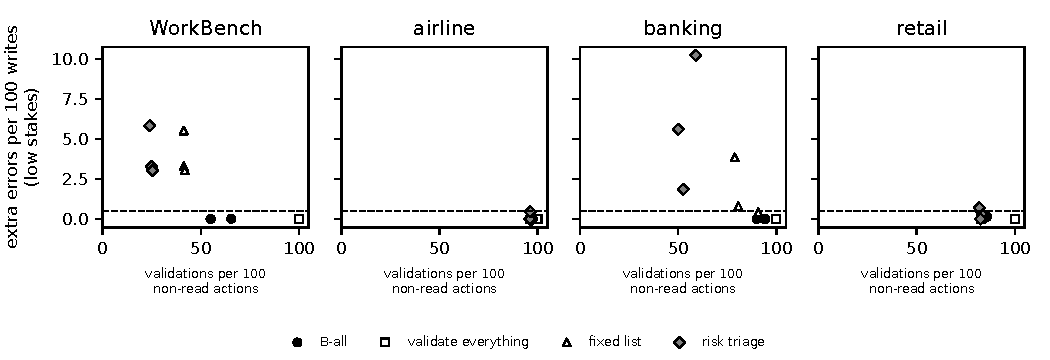
\includegraphics[width=1\linewidth,height=\textheight,keepaspectratio,alt={Validation load against extra errors at low stakes, per configuration, for B-all and the three comparators (descriptive: the pre-registered comparison is not judged). Dashed line: low-stakes budget.}]{../figures/fig3_load.pdf}
\caption{Validation load against extra errors at low stakes, per configuration, for B-all and the three comparators (descriptive: the pre-registered comparison is not judged). Dashed line: low-stakes budget.}\label{fig:load}
\end{figure}

\textbf{Secondary analyses (6.7).} In the main analysis, secondary rules had no established excess (B-regular had 4 under the delay10 stress test); the stress-test alert fired in all seven modes, driven by one airline cell carried by 2 tasks (worst upper bound 1.65 to 1.68 times the budget, 2.34 under delay10, 0 failures). Other secondary outputs (approve everything, three successes, oracle, order of episodes) are in Appendix C. Exploratory analyses, dated after the verdict (Appendix D): counting the 91 exclusions as errors adds one established type; the judgeable type stays above its bar with up to 63 \% false confirmations (Section 7). A second exploratory pass (Appendix D, Tables X7 and X8, dated 18 November 2026) read every confirmed plot error (\texttt{analytics.\allowbreak{}create\_\allowbreak{}plot}) of the judged type: 56 of its 79 errors are plots, and 48 of them differ from the expected action only by the end date (the agent plots up to 30 November, ``today'', where the benchmark expects 29 November). Across the study, the reviewing instances decided that end-date case both ways (177 such plot alerts lifted, 144 confirmed, all models and both halves). Lifting it throughout leaves 31 errors (3.4 \%, lower bound 0.86 \%), still established, but by two errors (29 are needed); lifting also four plots whose window is shifted by one day would leave 27, not established, and the label would become ``insufficient evidence''. The label R4 therefore depends on how one recurring, arguably acceptable discrepancy is judged.

\subsection{7 Discussion}\label{discussion}

R4 does not say that the agents are unreliable in general, that nothing could be delegated, or which model is better: it rests on one configuration, and only Haiku's volume made a type judgeable. Task success and action correctness also disagree: on WorkBench, 64 \% to 82 \% of episodes with a confirmed action error are successful tasks, and in every environment 47 \% to 77 \% of failed episodes have no confirmed action error (Table X7, exploratory). Failed episodes without a confirmed action error fail through reads, omissions or answers, which the action check does not count; on WorkBench, most errors inside successful tasks are the plot end-date case of Section 6.7, so this gap partly reflects the expected-path convention. What bound the study was volume, not the bound. At the budgets we fixed, the evidence the rule demands is out of reach at medium and high stakes for one benchmark configuration, and at low stakes for agents that err several percent of the time. Table X2 (exploratory) gives, for each established excess, the share of confirmed errors that could be false alerts before the excess is lost: 70 \% to 79 \% on retail money-moving writes, 31 \% to 55 \% on airline, 63 \% for the type that carries R4. The author's blind sample (3 of 10 confirmed alerts lifted, five per wave; 95 \% interval 7 \% to 65 \%, all environments pooled) is too small to rule such shares out: at its upper end, 9 of the 20 established excesses, including the one that carries R4, would no longer be established. Zhang and Zhang leave the evidence relation abstract; our rule is one instance; the budgets fix what it costs (Table 1), and our data show that agents erring several percent of the time could not pay it at these volumes. CASE ties autonomy to the remaining budget; our N is a different way, sized in advance per action type with a stated bound, and our data say nothing about CASE's mechanism. In practice, no type could have been delegated with evidence: 13 had no observed error but too few writes, 7 had errors without an established excess, and 20 had established excesses. Earning autonomy under such budgets takes tens to hundreds of verified successes at low stakes and thousands to tens of thousands at high stakes. A tier where actions execute then get flagged lowers load but lets errors through (about 4.6 to 6.2 errors per 100 writes of the type on WorkBench, exploratory). The extended version of this paper (see Appendix F) gives the full discussion.

\subsection{8 Limitations}\label{limitations}

Offline replay of fixed traces with a simulated validator; immediate detection; one expected path per task; tasks replayed up to 50 times; a simulated user that may drift; same-provider reviewers, blind by instruction only, with the wave-1 reviewing model not recorded and wave-2 batches closed in about 32 s each; a blind sample of 10 confirmed alerts, too small to bound false confirmations; an inconsistent review of a recurring plot end-date discrepancy that carries 48 of the 79 errors of the judged type, on which the label depends (Table X8); exclusions that favour delegation; insufficient volume at medium and high stakes; refused writes counted as errors; confirmed errors inside successful tasks (64 \% to 82 \% of the WorkBench episodes with a confirmed error); an audit of alert-free tasks too small to be informative (0 of 21 writes); one provider, three models, four environments. Appendix E lists all 32 limitations, each marked as pre-registered or added after the results, and Appendix A lists the 14 deviations from the pre-registration (D0 to D13), including an in-memory fix of a code defect in the final replay and the replacement of a verdict-freeze registration (OSF u26kr by cusv6).

\subsection{9 Conclusion}\label{conclusion}

On four public benchmarks and three Claude 5.5 models, none of the twelve configurations earned delegation: the only one that could be judged has an error rate established above its bar, and the other eleven lacked the effective volume to conclude. The rule was not refuted, but it was hardly put to the test, and its usefulness could not be judged. The errors counted are action errors confirmed against a single expected path per task, and 3 of 10 confirmed alerts in the author's blind sample were lifted. The main descriptive result is the delegation gap: the excesses these volumes could establish are large (lower bound 2.7 to 5.5 times the bar on WorkBench reversible writes), smaller gaps could not be resolved either way, and no type could be shown below its bar. As the plan stated in advance, earning autonomy under explicit budgets takes far more verified actions per action type than these benchmarks provide at our volumes. Code, data, registrations and the exact replay command will be public when the paper is posted (Appendix F).

\subsection{Acknowledgements and declarations}\label{acknowledgements-and-declarations}

\textbf{Use of AI tools.} Following arXiv's policy on authors' use of generative AI language tools (\url{https://info.arxiv.org/help/moderation/index.html}, read on 17 November 2026: authors must ``report in their work any significant use of sophisticated tools'', including text-to-text generative AI, and such tools ``should not be listed as an author''), we declare that Claude models (Anthropic), through Claude Code, were used, under the author's direction, to write the code of the instrument, the replay engine and the analysis scripts, to draft and revise the text of the plan, the registrations and this paper, to search and summarise the literature, and to audit the results and the paper. Claude also proposed, and in places settled, analysis choices recorded in the frozen plan (marked ``Tranché par Claude'' there; for example the order of labels and the max-T procedure); the author approved the plan as frozen. The audits and reviews cited in this paper were run by separate Claude instances, not by a third party. Separate Claude instances reviewed the automated alerts on blind sheets (Section B.4.3) and the alert-free tasks. The agents evaluated are also Claude models, from the same provider (limitation 9). The author takes full responsibility for all contents.

\textbf{Review.} Beyond the blind alert reviews and the automated audits described above, this paper has not had an external human review.

\textbf{Funding and competing interests.} The API costs (837.19 USD) were covered by credits from Anthropic's startup programme (Claude for Startups), granted to the author's micro-enterprise. The reviewing instances used a subscription paid by the author. Anthropic had no role in the design, conduct, analysis or writing of this study. The author runs a micro-enterprise, at proof-of-concept stage, that builds AI-agent services and uses Claude models among others.

\textbf{Availability and licences.} Code, frozen plan, registrations, replay outputs and the scripts that produce every table and figure will be public when the paper is posted (Appendix F; the OSF registrations are under embargo at the time of writing). The replay outputs were deposited on Zenodo on 17 November 2026, files under embargo until the paper is posted (doi:10.5281/zenodo.24321214); the code will be at \url{https://github.com/otsoa-dubief/earned-autonomy} and on Zenodo (doi:10.5281/zenodo.24331243), and the raw data, the 68,990 files of the verdict-freeze manifest, on Zenodo (doi:10.5281/zenodo.24331245); the text is released under CC BY 4.0 and the code under the MIT licence, as declared in the OSF deposits. τ-bench 2.0 and WorkBench are used under their MIT licences.

\textbf{Contact.} Otsoa Dubief, otsoa.dubief@gmail.com.

\begin{center}\rule{0.5\linewidth}{0.5pt}\end{center}


\nocite{*}
\bibliographystyle{unsrt}
\bibliography{refs}

\clearpage
\appendix
\subsection{A Deviations from the pre-registration}\label{a-deviations-from-the-pre-registration}

The plan was frozen at git tag \texttt{gel-2026-11-09} (commit a8eb1aae) and registered on OSF on 10 November 2026. Changes made before the freeze are declared in the registration itself: the two rule corrections, the redefinition of R4, the max-T formula, and others. They are listed in full in \texttt{JOURNAL\_\allowbreak{}CHANGEMENTS.\allowbreak{}md}. We list here what happened at or after the freeze. None of it changes the frozen files, the rule or the labels.

\begin{itemize}
\tightlist
\item
  \textbf{D0 (9 November, night, at the freeze): aborted freeze.} A first freeze commit (7e951f2) and its local tag, never published, were abandoned. A test of the frozen perimeter still checked the pre-freeze state (``G0 not drawn'') and failed once G0 was drawn. The test was corrected, the aborted outputs were removed by a new commit without rewriting history, and the freeze was redone with the same master seed G0. Already declared in the registration.
\item
  \textbf{D1 (10 November, evening): simplified page for the author's blind review, wave 1} (presentation, with effects on the task). The author found the frozen review page very hard to approach: too long, unclear about what to judge, in English and technical, as in the pilot. A simplified page, generated outside the frozen perimeter (\texttt{outils/\allowbreak{}relecture\_\allowbreak{}simple.\allowbreak{}py}) from the same blind sheets and the same draw, shows one sheet at a time, puts the field-by-field difference first, asks the four lift reasons as guided yes/no questions and folds the English evidence; it reads only the sheet number and alert ID from the draw, so no first-reviewer opinion appears, and its CSV output is read by the unchanged agreement script. It is not only a change of presentation: (i) the page computes the verdict from the four answers; (ii) it asks the reasons in the order b, c, a, d, with the default ``when in doubt, a real error''; (iii) question (a) omits three of the frozen rules for a defective task; (iv) question (d) is worded more loosely than the frozen reason. The frozen review page was never used by the author. No code in the frozen \texttt{banc/} directory was modified.
\item
  \textbf{D2 (10 November, evening): reading outside the pre-written list of between-wave checks, and a newly identified exclusion bias.} At the author's request, before launching wave 2, the error lines (\texttt{ERROR}, \texttt{Infra\ Errors}) of the logs of failed banking attempts were read, without any conversation content. All 19 failures had the same cause: τ-bench rejects an agent message that is empty, with neither text nor tool call, and classes it as an infrastructure error. This is agent behaviour counted as a technical failure. Under the frozen launcher such attempts are relaunched once, then excluded. This probably removes agent errors (banking, mostly Haiku) and biases results toward delegation, like the WorkBench bias already declared. Nothing was corrected, since the code is frozen. Recurrent \texttt{get\_\allowbreak{}response\_\allowbreak{}cost} messages (``LLM Provider NOT provided'') appear in all episodes, successful ones included, and have no effect. Final count: 91 episodes excluded, all for an empty agent message, 89 of them on banking (Table 3; D10).
\item
  \textbf{D3 (10 November, evening): wave-2 launch incident} (no effect on verdicts). Wave 2 was first launched outside a terminal multiplexer and interrupted within a minute (exit code 130). Two episodes were interrupted and replayed. It was resumed and then stopped by the launcher's guard (``incomplete or unreadable usage, cost marked up''). The cause: the resume path was given as a relative path, as in the launch notes. The launcher does not resolve it, so the per-episode usage file path became relative, while τ-bench runs in its own directory, and the cost counter wrote nothing. One finished episode (retail, Sonnet) has an upper-bounded cost of 0.174 USD; one attempt (airline, Haiku) became a technical failure (``usage absent'') and was replayed. The cumulated cost of the two attempts is 0.257 USD. Because the code is frozen, the launcher was not changed. Resumption uses absolute paths, tested in a dry run, and the launch notes were corrected accordingly.
\item
  \textbf{D4 (10 and 14 November): author's lifts outside any written reason.} In wave 1, the author lifted two sheets under reason (d) because the simulated client departed from its own instruction. No frozen reason covers this case ((d) is reserved for defects of our comparison code). Under the frozen rule the author's decision prevails and a reason is never rewritten, so these lifts enter the confirmed verdicts (the engine counts 3 alerts as lifted by the author without a written reason; the third, from wave 2, is not described here; no sensitivity analysis reconfirming these 3 of 2,761 alerts was run; Section C.6.1). This points to a real limitation of the benchmarks: a simulated client that drifts makes the agent who follows it look wrong (Appendix E).
\item
  \textbf{D5 (13 November): cost above the announced interval.} API spend reached 837.19 USD against a preregistered estimate of 595.73 USD (517 to 674 USD at 95 \%). Banking cost two to three times more per episode than in the pilot. No pass-count reduction was triggered (Section C.6.1).
\item
  \textbf{D6 (13 November): tools missing from the tool table} (instrument). The wave-2 report lists 27 banking tool names absent from the frozen tool table: 19 real tools, present in the frozen tool definitions but never mapped, and 8 \texttt{\_\allowbreak{}placeholder} names invented by the agent; 2 invented names appear on retail. Their writes stay without a verdict (\texttt{unknown}, tier 1) and explain banking's coverage (92.5 \% in wave 2; 98.5 \% overall in that wave, above the threshold). Nothing was corrected, since the code is frozen.
\item
  \textbf{D7 (13--14 November): alert review procedure for wave 2.} The 2,529 wave-2 alerts were reviewed in 1,428 batches by a script outside the frozen perimeter (\texttt{outils/\allowbreak{}relecture\_\allowbreak{}lots.\allowbreak{}py}), with the wave-1 prompt word for word. Each batch went to a fresh headless Claude Code instance on a subscription (no API key), without the author's personal settings, with the model recorded: Claude Opus 5.5. The wave-1 reviewing model and batching rule were not recorded. Wave-2 batches held at most 120 kB and 15 sheets; all 1,428 closed at the first attempt (about 2 h 05 with six instances in parallel). Reviewers could technically open the alert file, which the prompt forbade; no transcript was kept, so blindness rests on the instruction, not on a technical barrier. Opus 5.5 reviewed episodes played in part by Opus 5.5 (Appendix E, limitation 9). The harness of the wave-1 review was not recorded either, so the two waves were not reviewed under documented identical conditions. The analyses suggested by the audit of 14 November (lifts broken down by agent model, a review of a sample by another provider, re-reviewing wave 1 with the wave-2 harness) were not done.
\item
  \textbf{D8 (13 November): simplified review page reused in wave 2.} The simplified page of D1 also served for the author's wave-2 blind review, with the four guided questions in the order b, c, a, d and the default ``when in doubt, a real error''. The page computes the answer from four yes/no questions and invites the reader not to read everything, which may steer the reviewer; both wave-1 disagreements concerned question (d).
\item
  \textbf{D9 (14 November): audit of alert-free tasks.} The 20 audit sheets were read by a script outside the frozen perimeter (\texttt{outils/\allowbreak{}audit\_\allowbreak{}relecture.\allowbreak{}py}): one fresh Opus 5.5 instance per sheet, on the subscription, with the frozen instruction; the model is recorded. Result: 0 removals, 0 invisible errors in 21 writes.
\item
  \textbf{D10 (14 November): wave-2 exclusion diagnosis.} Reading only the error lines of the failed attempts' logs: of 226 technical failures in wave 2, 207 came from an empty agent message and 19 from an empty simulated-client message, a simulator failure (in wave 1, all 19 came from the agent). The exploratory analysis fixed in the verdict-freeze deposit counts only the former as errors. Final count of excluded episodes: 91 (Table 3).
\item
  \textbf{D11 (14 November): opposition on retail task 98, and a replaced verdict-freeze registration.} A first verdict-freeze registration (OSF u26kr, 06:44:26 UTC) was submitted. An audit by a separate Claude instance then found, before any draw, that retail task 98 had been removed on a consequence-based argument outside the frozen criterion (a recommendation error by the AI assistant, acknowledged), that the exact final-replay command was not fixed anywhere, and that the reference timestamp was ambiguous. The author opposed the removal of task 98, whose 23 alerts lifted for reason (a) became confirmed errors. u26kr could no longer be cancelled: its embargo had already been approved by the author on the assistant's instruction. The author chose to deposit a new registration (OSF cusv6, \texttt{date\_\allowbreak{}registered} 2026-11-14T08:17:47 UTC) declaring that it replaces u26kr and is the only one that counts, before the number designated by u26kr existed, then to withdraw u26kr (done). The draw designated by u26kr was never run. The three banking removals based on the knowledge base were kept; reading the policy's pointer to the knowledge base as part of the task's files is an interpretation of the frozen instruction, declared here. No sensitivity analysis keeping these three tasks was run. Banking task\_082, removed for case a3, was the least clear-cut removal.
\item
  \textbf{D12 (17 November): final replay, a code defect and its in-memory fix.} The final replay launched with the deposited command failed after 4,614 s while writing the stress-test table (\texttt{resistance.\allowbreak{}csv}): the frozen function \texttt{lignes\_\allowbreak{}resistance} passed two \texttt{mode} keys to the same record, a case that never arose in the pilot because no stress-test cell was judged there. The frozen code was not edited, since the engine refuses to run if the repository differs from the frozen manifest. Instead, a wrapper script (\texttt{outils/\allowbreak{}rejeu\_\allowbreak{}final\_\allowbreak{}correctif.\allowbreak{}py}) replaced that single function in memory, renaming the second field \texttt{mode\_\allowbreak{}scenario}, and called the engine's entry point with exactly the deposited arguments. Strictly speaking, this is therefore not the same command. The run metadata (\texttt{meta.\allowbreak{}json}) records the fingerprint of the frozen \texttt{sorties.\allowbreak{}py} and says nothing about the in-memory replacement; a separate note documents it. The replaced function only formats \texttt{resistance.\allowbreak{}csv}, which therefore has one extra column, and it is called after the label has been computed, so the label does not depend on it. No output of the first run was read before the second run; the six tables written by both runs are byte-identical, as checked by comparing SHA-256 fingerprints only (\texttt{revues/\allowbreak{}2026-11-17\_\allowbreak{}identite\_\allowbreak{}six\_\allowbreak{}tables.\allowbreak{}md}).
\item
  \textbf{D13 (17 November): tools and analyses after the verdict.} Presentation scripts outside the frozen perimeter were corrected or added after an audit of the results: \texttt{outils/\allowbreak{}tables\_\allowbreak{}article.\allowbreak{}py} (tables 3, 5, 6, 8, 9; only simple derived quantities such as counts, ratios and n\_eff × bar, never a new test), \texttt{outils/\allowbreak{}tables\_\allowbreak{}exploratoires.\allowbreak{}py} and a figure register (\texttt{article/\allowbreak{}sources\_\allowbreak{}chiffres.\allowbreak{}csv}). The exploratory analyses of Appendix D (\texttt{outils/\allowbreak{}analyses\_\allowbreak{}exploratoires.\allowbreak{}py}, A to G) were run after the verdict, read the frozen engine's outputs and functions without modifying them, are dated 17 November 2026, and have no effect on the label.
\end{itemize}

\begin{center}\rule{0.5\linewidth}{0.5pt}\end{center}

\subsection{B Rule and setup in detail}\label{b-rule-and-setup-in-detail}

\subsubsection{B.3 The earned-autonomy rule}\label{b.3-the-earned-autonomy-rule}

The rule is written in nine pieces (REGLE.md, frozen). We summarise the pieces that matter for the experiment. Where this summary and the frozen texts differ, the frozen texts prevail.

\paragraph{B.3.1 Unit of evidence: the action type and its stakes}\label{b.3.1-unit-of-evidence-the-action-type-and-its-stakes}

Actions are classified by what they do, not by the tool that performs them, through a frozen table that maps each benchmark tool to a type, a stakes level and reversibility (\texttt{banc/\allowbreak{}table\_\allowbreak{}outils.\allowbreak{}json}, v1). Each type has a single stakes level:

{\def\LTcaptype{none} % do not increment counter
\begin{longtable}[]{@{}ll@{}}
\toprule\noalign{}
Stakes & Types \\
\midrule\noalign{}
\endhead
\bottomrule\noalign{}
\endlastfoot
Low & read (no effect); reversible write; internal message \\
Medium & durable write; execution and delegation \\
High & external output; money; guardrail or rights; illegible effect \\
\end{longtable}
}

An action with two effects takes the higher stakes (cancelling an order also refunds it, so it counts as money). A tool absent from the table is treated as ``illegible effect'', at high stakes. Evidence stays within its type: successes on one type never count for another, and an error on one type does not freeze the others. Doubts raised by the agent (asking to transfer to a human) are neutral: they cost a validation but are neither a success nor an error.

Reads are autonomous from the start and enter neither the load nor the damage count; the instrument gives them no verdict. The budget is counted per \emph{write}. This is a declared second correction of the rule, made after the pilot showed that reads were 85--89 \% of actions in customer service. Counting per action made the bars absurd where writes are rare, and let an agent widen its own bar by reading more. Results are reported under both definitions (per write, primary; per action including reads, secondary).

\paragraph{B.3.2 Caps}\label{b.3.2-caps}

Some actions are always validated, whatever the evidence: modifying a guardrail or the agent's own rights, attesting the human's consent, revealing a secret. Money above a per-environment amount is also capped (2,500 USD in airline, 500 USD in retail, 400 USD in banking, roughly the top quarter of expected amounts), as is a first message to an unknown recipient. Only the human changes a cap, by a dated decision. The idea of a ceiling that evidence cannot lift follows Zhang and Zhang (2026); the amounts and the first-message cap are ours.

\paragraph{B.3.3 Tiers, promotion and withdrawal}\label{b.3.3-tiers-promotion-and-withdrawal}

There are three tiers: (1) \emph{ask before}: the write is validated before execution; (2) \emph{act then notify}: it executes, and the same validator can correct it afterwards (reversible types only); (3) \emph{act alone}. Irreversible types go directly from tier 1 to tier 3.

The main rule, \textbf{B-all} (named B-tout in the frozen plan), is applied per type, in the order of the sequence:

\begin{enumerate}
\def\labelenumi{\arabic{enumi}.}
\tightlist
\item
  tier 3 is reached after N consecutive verified successes on the type;
\item
  any error, at any tier, resets the run counter to 0;
\item
  an error at tier 3 withdraws autonomy. At medium or high stakes the type returns to tier 1 and a \emph{trial} opens; at low stakes it drops to tier 2 if reversible, tier 1 otherwise. Any medium- or high-stakes error opens a trial;
\item
  after a medium- or high-stakes error, the next climb requires ⌈1.25 N⌉ successes (``the error stays''); the lengthening does not accumulate;
\item
  the counter is frozen while a trial is open; a trial consists of three variants of the faulty case, and in the offline replay a variant is another recorded episode of the same task played by the current model. Trials are played ``dry'': they cause no damage and their validation load is counted separately. A failed trial imposes a wait of 50 writes of the type;
\item
  the counter is capped at the required length;
\item
  a model change (or extended rights) resets the counter. Remembered medium- and high-stakes errors become trials for the new configuration; low-stakes errors are dropped;
\item
  unverifiable writes and doubts are neutral: no success is ever assumed.
\end{enumerate}

Below tier 3, tier 2 of reversible types follows a Wald (1945) sequential score with fixed starting settings. Its parameters are (p\_good, p\_bad) = (0.10, 0.30) at low stakes and (0.05, 0.20) at medium stakes, with α = β = 5 \%.

An automated check judges each write; the agent never judges itself. An automated alert becomes an error only after confirmation (Section B.4.3).

\paragraph{B.3.4 From an error budget to N, and the guarantee}\label{b.3.4-from-an-error-budget-to-n-and-the-guarantee}

\textbf{Budget.} Blind, before seeing whether the corrected rule passed the synthetic simulation, the author fixed the extra errors he would accept relative to ``validate everything'', in exchange for fewer validations: 0.5 per 100 writes at low stakes, 0.05 at medium and 0.005 at high. Each level is ten times stricter than the one below. The order of magnitude was anchored, qualitatively, on human error rates for routine tasks in human reliability analysis (HEART, Williams, 1985; THERP, Swain and Guttmann, 1983), whose data are old and debated. We state no range from these sources.

\textbf{Bar.} The budget B\_ℓ of level ℓ is converted into a per-type error rate, the \emph{bar}, for each environment e:

bar(ℓ, e) = B\_ℓ / (0.95 × 100 × q(ℓ, e)),

where 0.95 is the share of errors the simulated validator stops (it misses 5 \%). q(ℓ, e) is the expected share of level-ℓ writes, computed from the expected actions of all tasks of the environment: the numerator excludes capped writes, the denominator includes all typed expected writes. A level with no expected write keeps a fallback bar from the synthetic exploration profile.

\textbf{Run length.} With d = 0.95 the assumed share of errors that the automated check detects, B-all uses

N = ⌈1 / (d × bar)⌉ − 1,

computed in exact fractions. A secondary rule, B-regular, uses the smallest N such that \(N^N/(N+1)^{N+1} \le d \times \mathrm{bar}\), which is enough for an agent with a constant error rate but not for arbitrary behaviour.

\textbf{Table 1. Bars and run lengths per environment} (frozen; bars rounded for reading; the configuration file holds exact fractions). Cell: bar (N for B-all; N for B-regular).

{\def\LTcaptype{none} % do not increment counter
\begin{longtable}[]{@{}
  >{\raggedright\arraybackslash}p{(\linewidth - 6\tabcolsep) * \real{0.2500}}
  >{\raggedright\arraybackslash}p{(\linewidth - 6\tabcolsep) * \real{0.2500}}
  >{\raggedright\arraybackslash}p{(\linewidth - 6\tabcolsep) * \real{0.2500}}
  >{\raggedright\arraybackslash}p{(\linewidth - 6\tabcolsep) * \real{0.2500}}@{}}
\toprule\noalign{}
\begin{minipage}[b]{\linewidth}\raggedright
Environment
\end{minipage} & \begin{minipage}[b]{\linewidth}\raggedright
Low stakes
\end{minipage} & \begin{minipage}[b]{\linewidth}\raggedright
Medium stakes
\end{minipage} & \begin{minipage}[b]{\linewidth}\raggedright
High stakes
\end{minipage} \\
\midrule\noalign{}
\endhead
\bottomrule\noalign{}
\endlastfoot
Airline & 1/12 (12; 5) & 1/194 (204; 75) & 1/12,020 (12,653; 4,655) \\
Retail & 1/38 (39; 15) & 1/697, fallback (733; 270) & 1/11,335 (11,931; 4,389) \\
Banking & 1/86 (90; 33) & 1/637 (670; 247) & 1/2,453 (2,582; 950) \\
WorkBench & 1/132 (138; 51) & 1/580 (610; 225) & 1/4,698, fallback (4,945; 1,819) \\
\end{longtable}
}

\textbf{Guarantee.} Consider one type at tier 3. Each autonomy period is preceded by at least N verified successes of that type and ends at the first detected error. Let d be the share of errors that the automated check detects after execution, independently of the agent's choices. Count in cycles: N successes, then errors until the first detected one, which takes 1/d errors on average, all executed. The expected number of errors executed at tier 3 per write of the type is then at most 1/(1 + N d), whatever the sequence of errors. This is the cycle argument of the unrestricted AOQL (1 − f)/(1 + if) of Lieberman (1953), with i = N and f read as d, without the factor (1 − f) in the numerator, because a detected error is not prevented: detection follows execution. If d = 1, the bound is deterministic: at most one executed error per N + 1 writes. If d \textless{} 1, it is a ratio of expectations per cycle, hence a long-run bound; on a finite sequence, the last, incomplete cycle is not covered by this statement. It falls if the errors the check misses are targeted. The preregistered N, drawn from N + 1 ≥ 1/(d × bar), is slightly conservative: since d ≤ 1, 1/(1 + N d) ≤ 1/(d (N + 1)) ≤ bar, so the simplification never weakens the guarantee. Summing over the types of a level, let s be the real share of non-capped writes of the level among the denominator writes, and q the expected share used for the bar. Two 0.95 factors must be kept apart: the validator's stop rate (1 − e, inside the bar) and the detection share d (inside N). With immediate and complete detection (d = 1 in the bound), the errors executed at tier 3 stay below budget × s/q per 100 writes, and, averaged over validator draws, the extra errors relative to ``validate everything'' stay below 0.95 × budget × s/q. This is the construction bound published for every cell (plan, 1.4). If only a share d = 0.95 of errors is detected, as assumed when N was computed, the expected executed errors stay below budget × s/(0.95 q) and the extra errors below budget × s/q: the budget still holds whenever s ≤ q, which is what the factor d in N buys.

\textbf{Assumptions.} The bound holds (i) for errors that the check detects, (ii) when detection is immediate, and (iii) relative to a validator that never rejects a correct write. If detection arrives k writes late, the bound becomes roughly (1 + k)/(N + 1) per write. An error that the check never sees is not covered: it counts as a success. N was computed with d = 0.95, and the bound holds in expectation over misses that are independent of the agent's choices; if misses are targeted (the agent errs exactly where the check is blind), no bound holds. The guarantee also does not cover tolerant variants, where a cycle may contain several detected errors. Finally, the bound is relative to the \emph{expected} mix q. If the real share s of a level exceeds q, the bound grows by s/q. For banking at low stakes, the pilot mix gives s/q ≈ 2.2, so the construction bound there is about 2.1 times the budget.

\textbf{Choice of B-all.} B-all was chosen over B-regular by the author on 4 November 2026, before the freeze. A synthetic exploration (E1, exploratory and deposited) had selected B-regular by a pre-written choice rule: lower validation load (63.8 against 72.7 per 100 non-read actions). But E1's robustness alert fired. With 10 \% of errors missed by the automated check, B-regular exceeded the budget in 9 cells (up to 1.05 times); with hard cases always missed, in 75 cells (up to 2.26 times). B-all's figures were 0 and 6 cells (up to 1.22 times). B-regular, and two Wald-based rules with p\_bad = bar and p\_good = bar/2 or bar/4 (A½, A¼), are replayed as secondary rules.

\begin{center}\rule{0.5\linewidth}{0.5pt}\end{center}

\subsubsection{B.4 Experimental setup}\label{b.4-experimental-setup}

\paragraph{B.4.1 Environments and tasks}\label{b.4.1-environments-and-tasks}

We use four environments from two public benchmarks: τ-bench 2.0 (\texttt{airline}, \texttt{retail}, \texttt{banking\_\allowbreak{}knowledge}; commit 033bf08) and WorkBench (commit 49c7dfd). Airline is graded with substring matching for communication and retail with forced state evaluation, so that no LLM judge is used. Banking uses BM25/grep retrieval without third-party calls. WorkBench uses all tools, structured outputs and logged traces, and has no simulated user. A development set of 20 \% of the tasks of each environment (stratified by file for WorkBench) was drawn on 5 November 2026. It was used for a pilot and for engine tests only; no development task enters the verdict. The reserved tasks are 40 (airline), 91 (retail), 77 (banking) and 552 (WorkBench).

\paragraph{B.4.2 Models and settings}\label{b.4.2-models-and-settings}

The agents are \texttt{claude-haiku-5-5}, \texttt{claude-sonnet-5-5} and \texttt{claude-opus-5-5}, called through the provider API with default settings. No temperature is set, since the API rejects it for these models. Default effort is medium for Haiku and Opus and high for Sonnet. The τ-bench simulated user is \texttt{claude-haiku-5-5} for all configurations. Prompt caching is enabled for τ-bench and unavailable for WorkBench's client. Each τ-bench episode is limited to 100 turns and 30 minutes. For each call, the launcher records the model name returned by the API and the tool definitions received by the agent; a change stops the run.

\textbf{Table 1 bis. Planned episodes} (frozen). A \emph{configuration} is one model in one environment (12 configurations).

{\def\LTcaptype{none} % do not increment counter
\begin{longtable}[]{@{}llllll@{}}
\toprule\noalign{}
Model & Airline & Retail & Banking & WorkBench & Episodes \\
\midrule\noalign{}
\endhead
\bottomrule\noalign{}
\endlastfoot
Haiku & 50 passes & 50 & 10 & 5 & 10,080 \\
Sonnet & 10 & 10 & 3 & 1 & 2,093 \\
Opus & 10 & 10 & 3 & 1 & 2,093 \\
\textbf{Total} & & & & & \textbf{14,266} \\
\end{longtable}
}

The estimated cost is 595.73 USD (approximate 95 \% interval 517--674 USD, reflecting pilot dispersion only), within a total research budget of 1,100 USD, pilot included. The independent unit is the task, not the episode.

\paragraph{B.4.3 The instrument: per-action verdicts and alert review}\label{b.4.3-the-instrument-per-action-verdicts-and-alert-review}

\textbf{Automated check.} Every write made with a tool of the frozen table is judged by exact comparison with the task's expected actions (\texttt{banc/\allowbreak{}verdicts.\allowbreak{}py}), without any LLM judge. A write is \emph{correct}, a \emph{duplicate}, \emph{refused} or \emph{wrong}. A duplicate with no extra effect on an idempotent tool is neutral; a duplicate that changes the state is an error. A write absent from the expected list is an error. A refused write is an error for the agent's record but not damage. A small number of comparison rules were adjusted on the pilot before the freeze, all logged. For example, payment\_id is compared only when a payment is actually recorded, and only the tool's name is compared when the agent gives a tool to the user. Task success rates, from each benchmark's final-state check, are reported alongside, because the check does not see work left undone.

\textbf{Alert confirmation.} An \emph{alert} is a write marked wrong, duplicate or refused. Every alert is reviewed by fresh Claude instances on blind sheets: no model name, episode number, rank or task identifier, only an opaque alert ID. Blindness holds for the sheets and is enforced by instruction, not by a technical barrier on the reading environment. In wave 2, the 2,529 alerts were reviewed in 1,428 batches by fresh Claude Opus 5.5 instances run headless through Claude Code on a subscription (each batch in its own instance, with only the project settings); the reviewing model was not recorded for the 232 alerts of wave 1. Coverage is published per environment. An alert can be lifted only for one of four reasons written in advance, with proof: (a) defective task; (b) mere rephrasing of a free-text field; (c) another path allowed by the policy that produces the user's intended effect; (d) a defect in our comparison code. Any other alert is confirmed. A task is \emph{defective}, and removed for all models and rules, only if its own files contradict each other: policy, initial data, simulated user's instruction, expected actions (four cases, a1--a4). An episode can signal a defect but never prove it. The author may oppose a removal before the verdict freeze; the task then stays and its alerts become confirmed errors.

\textbf{Blind human review.} In each wave, the author blind-reviews 15 alerts drawn at random (10 lifted, 5 confirmed, at most one per conversation), without the first reviewer's opinion. Agreement of at least 13 out of 15 keeps the review. Otherwise a second round of 15 is judged on both rounds (at least 26 out of 30). If that fails, the disagreement is persistent: no reason is rewritten after the freeze, and the label is computed twice, with retained decisions and with raw verdicts, keeping the less favourable one. If the first review lifted a real high-stakes error, all lifted high-stakes alerts are re-reviewed (plan 4.4).

\textbf{Audit of tasks without alerts.} After the last wave, five alert-free tasks per environment are read in full by blind Claude instances. Any write judged correct that the policy or the user's request contradicts is recorded as an ``invisible error''. This changes no verdict. It is published as a measure of what exact comparison misses.

\paragraph{B.4.4 Waves and spending caps}\label{b.4.4-waves-and-spending-caps}

Episodes are interleaved by relative rank, environment and model in an order drawn with a recorded seed, so that a stop leaves balanced coverage. Wave 1 is about 10 \% of each configuration (1,430 episodes, 60.53 USD estimated at pilot costs). It stops before any new episode at 80 \% of its cap, which is 1.5 times the wave estimate. Wave 2's cap is 1.25 times an estimate recomputed on wave 1, within the remaining budget. It stops at the smaller of 95 \% of the cap and the cap minus 15 USD. If 1.25 times the recomputed total exceeds the remaining budget, all pass counts are multiplied by the same factor, rounded down, with at least one pass per task and model. Technical failures are relaunched once, then excluded. Episodes stopped without a usable trace (WorkBench tool exception, context overflow, 35-minute kill) are excluded without relaunch and counted by configuration and reason. No episode is added in view of results. Between waves, only a pre-written list of checks is allowed (cost, run health, instrument coverage, alert review, defective tasks, returned model name). No rule replay, load, damage or error rate is computed before the final replay.

\paragraph{B.4.5 Calibration, confirmation and the public draw}\label{b.4.5-calibration-confirmation-and-the-public-draw}

The reserve is split by task, half and half, stratified by environment (and by file for WorkBench), within task pairs frozen before registration. The pairs are computed without randomness from expected actions, so that rare types are balanced. The \emph{calibration} half measures each configuration's confirmed error rate by type (Q2), supplies the oracle's rates and decides which configurations are delegable; the rule is never replayed on it. The \emph{confirmation} half is where the frozen rule is replayed, once, and where the verdict is read.

During collection the split does not exist, so no one can know which half a task belongs to. After the last wave, the confirmed verdicts and removed tasks are frozen, and their manifest is registered on OSF. The split seed is the SHA-256 of a fixed label, the manifest's hash and the first NIST Randomness Beacon pulse dated at least 72 hours after submission of that registration (an OSF registration can be withdrawn within 48 hours), with drand as a written fallback. Anyone can redo the draw from the public pulse and the registered hashes. The final replay then runs once, from one script, which refuses to start if the repository differs from the frozen manifest.

\paragraph{B.4.6 Offline replay}\label{b.4.6-offline-replay}

The rule and its comparators are replayed on the recorded episodes. For a configuration and a task set, episodes are shuffled, their write actions laid end to end, and reads and preparations removed. Every rule then sees the same sequence and the same validator draws (one uniform draw per write). At tier 1 an error passes if the draw falls below e = 5 \%; at tier 2 it executes and is corrected unless the draw falls below e; at tier 3 every error is damage. \emph{Extra errors} are errors executed at tier 3 that ``validate everything'' would have stopped, per 100 writes, per stakes level. The \emph{validation load} counts tier-1 validations (capped writes included), tier-2 corrections and doubts, per 100 actions excluding reads and preparations. Point estimates are means over R0 = 2,000 replays without resampling. Model-change scenarios concatenate the confirmation sequence of model X with that of model Y. There are 6 ordered pairs per environment, each in two modes: \emph{announced} (reset at the junction) or \emph{silent} (no event, which also serves as the ``no reset'' comparator). This gives 48 sequences. All sub-seeds derive from one master seed drawn at the freeze.

\begin{center}\rule{0.5\linewidth}{0.5pt}\end{center}

\subsection{C Pre-registered analysis and results in detail}\label{c-pre-registered-analysis-and-results-in-detail}

\subsubsection{C.5 Preregistered analysis}\label{c.5-preregistered-analysis}

This section restates the registered analysis plan. It adds nothing to it.

\paragraph{C.5.1 Cells and comparators}\label{c.5.1-cells-and-comparators}

A \emph{cell} is a configuration or a model-change sequence at one stakes level: (12 + 48) × 3 = 180 cells. The mandatory comparators are: \textbf{validate everything} (every write at tier 1; the reference for extra errors); the \textbf{fixed list} (reads and reversible writes at tier 3, everything else at tier 1); and \textbf{risk-based triage} (all low-stakes types at tier 3, the rest at tier 1). Reported without effect on the label: approve everything; autonomy after three successes; random delegation at the same rate as the rule, type by type; an oracle that delegates a type if its median calibration rate is at most the bar; a retrospective oracle; and the secondary rules (B-regular, A½, A¼).

\paragraph{C.5.2 Criteria and labels}\label{c.5.2-criteria-and-labels}

\textbf{Point 0, instrument validity.} Each wave ended with its blind review kept, or followed the persistent-disagreement rule. The coverage of the instrument (share of writes with a verdict) must be at least 0.95. Otherwise the label is R5, and everything is still computed and published.

\textbf{H1, safety (eliminatory).} B-all keeps the budget in every cell. A cell fails only if its excess is \emph{established} by the max-T procedure (Section C.5.3). Cells where B-all never reaches tier 3 in any of the R0 replays are ``held, not put to the test'' and leave the max-T family. A failure gives R1. The withdrawal criterion (at most one detected error before withdrawal at medium and high stakes) holds by construction under immediate detection. It is checked as a code control, not as a route to refutation; its delayed-detection version is reported.

\textbf{Delegable configuration.} A configuration is delegable if at least one earned type has a median calibration rate at most its bar. The median rate is the one-sided 50 \% Clopper--Pearson bound on the effective size. A type is \emph{judgeable} if zero errors would bring its median rate under its bar.

\textbf{No delegable configuration.} If no configuration is delegable, the label is R4 (preregistered name: ``nothing to delegate: unreliability established''; Section 7 and limitation 21 state what it means here) only if (i) at least one type is judgeable, and (ii) every configuration with a judgeable type has at least one judgeable type whose one-sided 95 \% Clopper--Pearson lower bound at ρ = 1 lies above its bar. Otherwise it is ``insufficient evidence'', with its reason: no judgeable type; excess not established; or excess established only under the configuration's own estimated correlation, not at ρ = 1.

\textbf{H2, utility.} With the budget kept, B-all must beat each mandatory comparator. ``Validate everything'' is beaten only on load: B-all's mean load over delegable configurations (equal weights) must be lower, with the paired-difference interval entirely and strictly below 0. The fixed list and the triage are beaten either by an established budget excess in at least one cell, or on load in the same way. Otherwise the label is R2. A rule that delegates nothing therefore cannot be confirmed: a competitor's fault is never a win.

\textbf{Final label}, in order of precedence: \textbf{R5} (instrument insufficient), \textbf{R1} (rule refuted), \textbf{insufficient evidence}, \textbf{R4} (preregistered name ``nothing to delegate''; see Section C.6.2), \textbf{R2} (safe but not useful), \textbf{confirmed} (H1 and H2 hold, with at least one delegable configuration).

\textbf{What R1 and ``confirmed'' can and cannot mean (plan 1.4).} With immediate detection, B-all's bound holds for any sequence: every error executed at tier 3 follows at least N successes of the same type, so at a given level the executed errors stay below budget × s/q per 100 writes, and the extra errors, averaged over validator draws, below 0.95 × budget × s/q. H1 can therefore hardly fail through the data. R1 can mean a mix gap (s above about 1.05 × q at a level where B-all reaches tier 3); it cannot mean, on its own, that the agents are unreliable, since B-all withdraws autonomy at the first error. The withdrawal criterion holds by construction and cannot refute the rule. ``Confirmed'' requires that B-all delegate in an established way with fewer validations than ``validate everything'', and that the risk triage be beaten by an established excess (where the triage keeps the budget, it necessarily asks for fewer validations than B-all); it cannot mean that B-all is safe at levels where it delegated nothing (``held, not put to the test''), nor beyond these benchmarks, models and settings. The part of the study that can really fail through the data is H2, together with the measured delegation gap.

\textbf{Q2, delegation gap (descriptive).} For each configuration and type, on the calibration half, we report: the error rate p = x/n (confirmed errors, refused included, over verifiable non-neutral writes); p/bar and upper bound/bar; the class (below the bar, above, indeterminate) at ρ = 1 and under the estimated \ensuremath{\hat{\rho}}; the median rate; whether the type is judgeable; and the certification volume. Under R4 or insufficient evidence, the delegation gap becomes the main result.

\textbf{Random delegation (separate conclusion).} If B-all lets through fewer extra errors than random delegation at the same rate at one level at least and more at none, autonomy is called \emph{earned}. If the difference is not shown, it is only \emph{distributed}. If neither has extra errors, the comparison is \emph{without object}. This comparison does not affect the label.

\paragraph{C.5.3 Intervals and multiplicity}\label{c.5.3-intervals-and-multiplicity}

The independent unit is the task. Intervals on load differences, on means over delegable configurations, on the comparison with random delegation and on proportions use a task-level jackknife-t (Student quantile with G − 1 degrees of freedom). It was selected before the freeze by a coverage simulation over ρ ∈ \{0, 0.1, 0.3, 0.5, 0.7, 0.9\} and G ∈ \{20, 40, 90\} task clusters, with a worst coverage of 0.933 against a 0.93 threshold. That coverage was measured on paired load differences (Monte-Carlo error about 0.35 point); on the budget cells, an earlier simulation had given the jackknife-t a worst coverage of 0.549, which is why the safety test uses max-T (plan 5.13). Intervals on extra errors are therefore nominal 95 \% intervals, read descriptively.

An \emph{established excess} uses a Westfall--Young max-T over the family of testable cells. It is fed by a stratified task-cluster bootstrap with B = 2,000 replicates, each averaged over K = 10 orders and validator draws. The statistic T*\_c is centred on the bootstrap mean and standardised by the cell's bootstrap SD. The critical value c* is the 97.5th percentile of the maximum over testable cells, floored at 0 (formula F3). An excess is established in cell c if estimate\_c − c* × SD\_c exceeds the budget. A cell is not testable if it has fewer than two carrying tasks, an undefined estimate, an undefined bootstrap SD, or a zero SD (within four float32 epsilons). Non-testable cells establish nothing and are published with their reason.

The nominal family-wise level is 5 \%, one-sided. The level measured before the freeze is 4.7 \% cumulated (28/600, Wilson 3.2--6.7 \%). It was measured in a synthetic world with all testable cells at their budget boundary, the least favourable configuration measured, not the worst possible world. Its interval exceeds 5 \%, so the measurement does not show that F3 holds 5 \%. It was measured with B = 200, not 2,000, and is not measured for the comparators. Tested alone, the worst low-stakes WorkBench cell is falsely declared in excess in 27 of 200 replicates. If the family has one or two testable cells, the max-T is almost an uncorrected test, and the output says so. The nominal risk of declaring the fixed list beaten wrongly can reach 7.5 \% (5 \% max-T plus 2.5 \% load interval). The choice of F3 is itself a declared deviation. The pre-set formula-choice rule, applied to the measurement draws only, designated F1, which over-rejected when all draws of the same quantity were counted (6.7 \%, 40/600); the rule was then applied to all draws and retained F3.

A cell is ``demonstrated'' if its one-sided 95 \% Clopper--Pearson upper bound on the effective sample size at ρ = 1 is at most the budget. At the planned volumes we expect few or no such cells. At zero damage, demonstrating 0.5 per 100 writes needs at least 598 independent writes, and errors cluster within tasks. The experiment can therefore refute the budget for B-all, but cannot demonstrate it configuration by configuration. Where no excess of B-all is established, its compliance rests on the construction bound and on the absence of an established excess.

\paragraph{C.5.4 Secondary and stress analyses (no effect on the label)}\label{c.5.4-secondary-and-stress-analyses-no-effect-on-the-label}

These analyses are: safety on the whole reserve; role swap (two-fold cross-validation); the secondary rules; the pre-freeze choice rule reapplied on the confirmation half; and raw verdicts (a verdict that changes between raw and confirmed is marked \emph{fragile}). Stress tests: 10 \% of confirmed errors unseen (miss10); evidence delayed by 10 writes (delay10); all errors of 10 \% of tasks unseen; and validator miss rates e = 0, 2 and 10 \%. We also report the budget per action (reads included), load with trials, and sensitivity to episode order. If plan text and frozen code diverge, the frozen code performs the confirmatory computation, and the text-based computation is published as exploratory.

\begin{center}\rule{0.5\linewidth}{0.5pt}\end{center}

\subsubsection{C.6 Results}\label{c.6-results}

\paragraph{C.6.1 Data collection and instrument}\label{c.6.1-data-collection-and-instrument}

\textbf{Episodes.} The plan called for 14,266 episodes; all were played, and 13,623 are analysed after exclusions and task removals (\texttt{reussite\_\allowbreak{}taches.\allowbreak{}csv}). Wave 1 stopped as designed at 80 \% of its cap (72.10 \$ cumulative when the stop triggered, against a 72.00 \$ stop; the cap was 90.00 \$, the amount the author approved, within the 90.78 \$ the plan allowed), after 1,185 episodes; the 13,081 not yet played moved to wave 2, which played all of them without any stop (wave reports, \texttt{rapport\_\allowbreak{}vague.\allowbreak{}txt}). No pass-count reduction was needed: 1.25 times the wave-2 estimate fitted in the remaining budget. Episodes stopped at the 100-turn guard were kept (4 in wave 1, 15 in wave 2, 10 of them Opus on banking).

\textbf{Exclusions (Table 3).} 91 episodes were excluded after one relaunch, all for the same cause: an empty agent message that τ-bench records as \texttt{infrastructure\_\allowbreak{}error} (9 in wave 1, 82 in wave 2). 77 of them are Haiku on banking (about 10 \% of Haiku's banking episodes), 10 Sonnet on banking, 2 Opus on banking and 2 Sonnet on airline. No episode was excluded for a WorkBench tool exception, a context overflow, the 35-minute guard or a change of the returned model name; that name never changed (about 209,000 calls in wave 2, none without a name in wave 1). These exclusions remove agent failures and therefore favour delegation; Appendix D counts them as errors (exploratory; established excesses go from 20 to 21).

\textbf{Cost.} API spend was 837.19 \$ (wave 1: 72.13 \$ once the episodes running at the stop had finished; wave 2: 765.07 \$), above the preregistered estimate of 595.73 \$ (517 to 674 \$ at 95 \%). The excess comes from banking, two to three times more expensive per episode than in the pilot. The pilot cost 14.77 \$. Alert review and the audit of alert-free tasks ran on a subscription, not on the API key (API-equivalent cost of the wave-2 alert review: 883.50 \$).

\textbf{Instrument coverage (point 0).} 98.68 \% of writes received a verdict, against a threshold of 95 \% on the whole set; every unverifiable write is an \texttt{unknown} write on banking, whose effect cannot be read. Coverage on banking alone was 93.0 \% in wave 1 and 92.5 \% in wave 2, below 95 \%; it is published per environment and listed as a limitation (Appendix E). In wave 2, the banking agent called 27 tool names missing from the tool table (19 real tools, 8 invented \texttt{\_\allowbreak{}placeholder} names); they stayed at tier 1, without a verdict.

\textbf{Alerts.} 2,761 alerts were reviewed one by one, none left without a decision: 1,991 confirmed as errors and 770 lifted, by reason a (defective task) 75, b 78, c 331, d 283, plus 3 lifted by the author outside any written reason (\texttt{decision.\allowbreak{}csv}). Twelve defective tasks were removed with all their actions (6 retail, 5 banking, 1 airline); the author opposed two candidate removals (WorkBench \texttt{multi\_\allowbreak{}domain:179}, retail \texttt{98}), whose alerts therefore count as confirmed errors.

\textbf{Blind human review.} In each wave the author re-reviewed 15 alerts drawn blind (10 lifted, 5 confirmed): agreement 13 of 15 in wave 1 and 13 of 15 in wave 2, at the threshold of 13; the review was kept both times and no second round was needed. In the four disagreements the author's decision replaced the first review; in the one where the author confirmed a lifted alert, the alert was not high-stakes, so the full re-review of lifted high-stakes alerts was not triggered (\texttt{accord.\allowbreak{}json} of each wave). Wave-2 alerts were first reviewed by fresh Claude Opus 5.5 instances, in 1,428 batches.

\textbf{Audit of alert-free tasks.} 20 alert-free tasks (5 per environment) were read by fresh reviewers: 0 invisible errors in 21 writes read (WorkBench 0/8, airline 0/3, banking 0/4, retail 0/6) and no defective task. With 21 writes, the upper bound stays near 13 \%; this audit is weak evidence.

\textbf{Symmetry between halves (Table 4).} The two halves hold the same number of tasks in each environment, within one task (WorkBench 276/276, airline 20/20, banking 38/39, retail 45/46). Removed tasks fall on both halves (calibration 6, confirmation 6). Writes per stakes level differ more: on airline, the confirmation half has 1,166 high-stakes writes against 542.

\textbf{Task success.} Task success varies far more by environment than by half: from 94.9 \% to 99.3 \% on WorkBench, 81.7 \% to 92.5 \% on airline, 84.0 \% to 92.8 \% on retail, and 18.3 \% to 50.9 \% on banking (per model and half; full table in Appendix C).

\textbf{Public draw.} The verdict freeze was registered on OSF (cusv6) on 14 November 2026 at 08:17:47 UTC. The designated NIST beacon pulse, the first at or after 72 hours later, is pulse 2031457 (17 November 2026, 08:18:00 UTC); its value seeded the task split, and the split file records the hash of the frozen manifest (\texttt{904aa8d3…f88d}). The split was recomputed and checked before the replay (Appendix F).

\paragraph{C.6.2 Preregistered label}\label{c.6.2-preregistered-label}

\textbf{Label R4.} No configuration reached the pre-registered level of evidence required for delegation. Only one of the twelve configurations had enough volume to be judged (Haiku on WorkBench, reversible writes, ECR); its confirmed error rate, 8.6 \% (914 writes, 79 errors; one-sided 95 \% Clopper--Pearson lower bound 4.1 \% at ρ = 1), is established above its 0.76 \% bar. The other eleven configurations have no judgeable type: their volume does not allow a conclusion either way. The lower bound is computed per action type, without correction for the twelve configurations (frozen rule); the gap with the bar, more than fivefold, makes chance an unlikely explanation, but no multiplicity correction was applied.

The judgeability of that single type is narrow: n\_eff × bar = 0.740 against a threshold of 0.6905 (about ln 2), with \ensuremath{\hat{\rho}} = 0.819; the type would stop being judgeable above \ensuremath{\hat{\rho}} = 0.885, and the label would then become ``insufficient evidence'' (Appendix D, Table X6, exploratory, gives an approximate bootstrap interval; it uses a simpler estimator than the engine's, pooled over types, so its share of draws above 0.885 likely understates the risk). At ρ = 1 the type would not be judgeable (n\_eff = 81.6, product 0.618): the judgeability rests on \ensuremath{\hat{\rho}}, as the plan specifies (5.13, N3).

\textbf{Decision table (Table 2, from \texttt{decision.\allowbreak{}csv}).}

{\def\LTcaptype{none} % do not increment counter
\begin{longtable}[]{@{}
  >{\raggedright\arraybackslash}p{(\linewidth - 2\tabcolsep) * \real{0.5000}}
  >{\raggedright\arraybackslash}p{(\linewidth - 2\tabcolsep) * \real{0.5000}}@{}}
\toprule\noalign{}
\begin{minipage}[b]{\linewidth}\raggedright
point
\end{minipage} & \begin{minipage}[b]{\linewidth}\raggedright
result
\end{minipage} \\
\midrule\noalign{}
\endhead
\bottomrule\noalign{}
\endlastfoot
0. Instrument validity & held: coverage 0.9868 (threshold 0.95); blind review kept in both waves \\
1. Eliminatory criterion (B-all, established excess by max-T) & held: 180 cells, 51 judged (6 of them non-testable: 5 with fewer than 2 carrying tasks, 1 without bootstrap variation), 108 held but not put to the test, 21 without object; 0 established excesses; 0 cells demonstrated below budget \\
Code control: withdrawal criterion of decision 5 & held: 0 periods with more than one confirmed error \\
2. Witnesses & not judged (no delegable configuration). For reference, ``validate everything'' has no cell at risk; the fixed list and the risk-sorted list have an established excess in 9 and 18 of 60 cells \\
3. Chance at the same pace & not computable (no delegable configuration) \\
4. Delegable configurations & none; in the only configuration with a judgeable type, its excess is established (R4) \\
6. Secondary analyses & raw verdicts: R4; whole reserve, point 1: held; role swap: R4; original letter (Q8 A), point 1: held; 0 cell disagreements in each \\
\end{longtable}
}

\textbf{``Fragile'' mentions.} 27 cells carry the ``fragile'' mention because they rest on fewer than 30 carrying tasks: five configurations (airline/Haiku, the three retail configurations, banking/Sonnet) and 22 model-change scenarios on airline and retail. The type that carries R4 rests on 134 carrying tasks.

\paragraph{C.6.3 Safety (H1)}\label{c.6.3-safety-h1}

\textbf{What ``held'' means here.} Point 1 is held in the sense of ``not refuted'', with almost no power: no established excess; the test could establish almost nothing (c* = 7.0, so an estimate would have had to lie more than seven standard errors above the budget); no cell demonstrated. H1 can hardly fail through the data. In the replay, every confirmed error at tier 3 is noticed at once, so the bound is deterministic (at most one executed error per N + 1 writes of the type), and the budget can only be exceeded if the actual share s of the type's writes exceeds the expected share q by about 5 \% (plan 1.4). That condition (s/q above 1/0.95) holds for the point estimate in 24 of the 51 judged cells, on WorkBench and banking. Of the two hypotheses, the one the data could really refute is H2, measured by the delegation gap (Section C.6.4).

\textbf{Table 5 (summary; full table with the result tables).} Of the 180 cells (12 configurations and 48 model-change scenarios, × 3 stakes levels), 21 are without object, 108 held but not put to the test, and 51 judged, all at low stakes. All max-T bounds are negative. In the 51 judged cells, the central estimate of extra errors stays at most 0.38 times the budget; a single descriptive upper bound lies above the budget (1.67 times; airline, Sonnet replaced silently by Opus, 2 carrying tasks).

\textbf{Figure 1} (\texttt{article/\allowbreak{}figures/\allowbreak{}fig1\_\allowbreak{}budget.\allowbreak{}pdf}) plots the extra errors per 100 writes against the budget for the 51 judged cells (filled: configurations; hollow: model-change scenarios), by environment and model.

\textbf{Withdrawal criterion.} As a code control, the withdrawal criterion of decision 5 passed in all 100 B-all rows of the main analysis in \texttt{derive.\allowbreak{}csv}: no period had more than one confirmed error (the maximum observed was 0). The delay10 version (detection delayed by ten writes) gives the same result.

\paragraph{C.6.4 Delegation gap (Q2)}\label{c.6.4-delegation-gap-q2}

The delegation gap compares, per configuration and action type, the confirmed error rate on the calibration half with the type's bar. Classes are computed at ρ = 1, conservative under an exchangeable within-task correlation and under the effective-size approximation (non-integer effective size and a beta law); a simulation run on the engine before any data found that this rule returns R4 wrongly at most 2.8 \% of the time at the bar (\texttt{REGLE.\allowbreak{}md}, amendment of 7 November). No multiplicity correction is made over the 40 types. At these volumes the table can only return ``above the bar'' or ``undetermined'': the plan stated in advance (5.13) that no type could be proven below its bar, so the count ``20 above, 0 below'' is partly built in. Only one type is judgeable (judgeability uses n\_eff under \ensuremath{\hat{\rho}}, Section C.6.2), and only that type bears on the label; the other classes are descriptive. Full table: Table 6, with the result tables; Figure 2 (\texttt{article/\allowbreak{}figures/\allowbreak{}fig2\_\allowbreak{}gap.\allowbreak{}pdf}) shows rate/bar with the ρ = 1 interval on a log scale; zero rates are drawn hollow at 0.001, and types with fewer than 5 writes (banking/Haiku ILL, 2 writes; banking/Opus GAR, 3) are marked.

\textbf{Overview.} 40 types have data. 20 are above their bar at ρ = 1, 20 undetermined, none below. Of the 20 undetermined types, 13 have no observed error: on WorkBench, Opus and Sonnet internal messages (MSG, 0 of 58 each) and medium-stakes writes (DUR, 0 of 106 each); on airline, reversible writes (ECR) for Haiku (0 of 67), Opus and Sonnet (0 of 20 each), and medium-stakes writes for Opus and Sonnet (0 of 20 each); on banking, irreversible high-stakes writes (GAR) for all three models (0 of 10, 3 and 6); on retail, Sonnet's reversible writes (0 of 122). Absence of observed errors on so few writes says nothing in favour of delegation.

Rates and their ρ = 1 bounds come first below, then the ratios, level by level. The ratio ``lower bound ÷ bar'' is the proven quantity; ratios of the rate itself to the bar mostly reflect how low the bar is.

\textbf{Low stakes, outside banking.} On WorkBench, reversible writes have an error rate established above the 0.76 \% bar for all three models: Haiku 8.6 \% {[}4.1 ; 15.6{]} (two one-sided 95 \% bounds, a 90 \% interval; 914 writes; lower bound ÷ bar 5.5; the judgeable type), Sonnet 6.1 \% {[}2.4 ; 12.5{]} (181 writes; 3.1) and Opus 5.5 \% {[}2.0 ; 11.7{]} (182 writes; 2.7). Low-stakes types on airline and retail are undetermined: retail reversible writes run at 3.2 \% (Haiku, 632 writes) and 3.8 \% (Opus, 132) against a 2.6 \% bar, with lower bounds at zero.

\textbf{High stakes, outside banking.} On airline, money-moving writes (ARG) have a rate established above the 0.0083 \% bar for the three models: Haiku 13.3 \% {[}0.6 ; 50.7{]} (308 writes; lower bound ÷ bar 70), Sonnet 11.1 \% {[}0.3 ; 47.3{]} (72; 39) and Opus 8.5 \% {[}0.1 ; 44.6{]} (71; 10). For Opus the excess is thin: 6 errors in 9 carrying tasks, lower bound 0.09 \%. On retail, the same type is established above its 0.0088 \% bar for Haiku 9.2 \% {[}2.2 ; 23.6{]} (2,511 writes; 248), Sonnet 6.7 \% {[}1.0 ; 20.5{]} (496; 118) and Opus 6.5 \% {[}1.0 ; 20.5{]} (492; 109). At these bars a single error in 500 writes already gives a rate/bar ratio of about 20, and certifying the type would take 33,956 to 36,009 consecutive verified successes (plan 1.4): the high-stakes ratios are a fact about the budget chosen as much as about the agents. The rates themselves are the informative quantity, but they come from the calibration half: on the confirmation half the same types err 1.2 \% to 7.7 \% (3.8 \% to 8.0 \% on the whole reserve), the two halves differing by up to a factor of five, and the intervals above are wide.

\textbf{Banking, apart.} Banking rates are high: established above the bar for money-moving writes at 53.5 \% (Haiku, 202 writes), 47.5 \% (Opus, 80) and 56.0 \% (Sonnet, 75); for medium-stakes writes at 44.9 \%, 28.5 \% and 41.4 \%; for internal messages at 27.7 \% (Haiku), 8.1 \% (Opus) and 11.3 \% (Sonnet); and for Sonnet's reversible writes at 32.6 \%. They are consistent with task success of 18 \% to 51 \% on this benchmark, but banking is also where attribution to the agent is weakest: coverage 0.925, 19 real tools missing from the tool table, a knowledge base not shown to reviewers (so defective tasks could not be lifted), high stakes carried by the simulated client, and 89 of the 91 excluded episodes. These rates therefore do not separate agent error from setup error. Two banking excesses are marginal: Opus internal messages are established by 0.3 \% (lower bound 1.165 \% against a 1.161 \% bar), and Haiku's ILL type rests on 2 errors in 2 writes.

\textbf{Correlation.} The estimated within-task correlation \ensuremath{\hat{\rho}} (stratified Fleiss--Cuzick) is 0.819 for WorkBench/Haiku, 1.0 for WorkBench Opus and Sonnet, 0.40 on airline, 0.40 to 0.47 on banking and 0.40 to 0.43 on retail; it is the larger of a floor (0.3) and the value pooled over all configurations, unless a configuration with at least 10 errors in at least 5 tasks has a larger value of its own (plan 5.13, N3). Every type established at ρ = 1 stays established under \ensuremath{\hat{\rho}}. One type changes class under \ensuremath{\hat{\rho}}: banking/Opus reversible writes (16.2 \%, 74 writes) would be established above its bar for any ρ ≤ 0.924, against \ensuremath{\hat{\rho}} = 0.431 (21 types above under \ensuremath{\hat{\rho}}).

\textbf{Delegable configurations.} None. The only configuration with a judgeable type, WorkBench/Haiku, has that type established above its bar; the label is R4 (Section C.6.2).

\textbf{Whole reserve (descriptive, not a label).} The preregistered label is computed on the calibration half; pooling both halves can only be descriptive (Table 6 bis: 22 of 41 types above, none below). With roughly twice the volume, three configurations would have had a delegable type, all with zero observed errors: internal messages for Opus and Sonnet on WorkBench (0 errors in 120 writes each) and reversible writes for Sonnet on retail (0 in 258). Elsewhere the pooled rates can differ from the calibration rates by a factor of one to five; for instance, Haiku's reversible writes on retail show 31 errors in 1,286 writes (2.4 \%, below a 2.6 \% bar but not provably so). This pooled view shows where more volume could have changed the picture; it does not change the label, which the preregistration ties to the calibration half.

\textbf{Exploratory, dated 17 November 2026 (not preregistered; Appendix D).} Counting the 91 excluded episodes as errors adds 24 errors on the calibration half, all on banking, and one more established type (21 instead of 20), resting on 5 writes (Table X1). Allowing a share of the confirmed errors to be false alerts, the judgeable WorkBench/Haiku type stays above its bar with up to 63 \% false confirmations, while banking/Opus internal messages would not withstand a single one (Table X2).

\textbf{Exploratory, dated 18 November 2026 (not preregistered; Appendix D, Tables X7 and X8).} A second exploratory pass read every confirmed plot error (\texttt{analytics.\allowbreak{}create\_\allowbreak{}plot}) of the judged type: 56 of its 79 errors are plots, and 48 of them differ from the expected action only by the end date (the agent plots up to 30 November, ``today'', where the benchmark expects 29 November). Across the study, the reviewing instances decided that end-date case both ways (177 such plot alerts lifted, 144 confirmed, all models and both halves). Lifting it throughout leaves 31 errors (3.4 \%, lower bound 0.86 \%), still established, but by two errors (29 are needed); lifting also four plots whose window is shifted by one day would leave 27, not established, and the label would become ``insufficient evidence''. The label R4 therefore depends on how one recurring, arguably acceptable discrepancy is judged. Task success and action correctness also disagree: on WorkBench, 64 \% to 82 \% of episodes with a confirmed action error are successful tasks, and in every environment 47 \% to 77 \% of failed episodes have no confirmed action error (Table X7, exploratory). Failed episodes without a confirmed action error fail through reads, omissions or answers, which the action check does not count; on WorkBench, most errors inside successful tasks are the plot end-date case above, so this gap partly reflects the expected-path convention.

\paragraph{C.6.5 Utility (H2)}\label{c.6.5-utility-h2}

\textbf{Point 2 is not judged.} Under R4 the plan does not judge point 2 (5.14, Q15): the comparison with the witnesses is defined as an equal-weight mean over delegable configurations, and there are none. For the same reason the reduction of validations against ``validate everything'' as a share of the oracle's gain, and the paired differences, are not computable. ``Validate everything'' is not beaten. (The detail of the ``point 2: success'' line in \texttt{decision.\allowbreak{}csv}, ``the three witnesses beaten'', is the wording of the criterion written into the engine's output, not a result.) Figure 3 (\texttt{article/\allowbreak{}figures/\allowbreak{}fig3\_\allowbreak{}load.\allowbreak{}pdf}) is therefore descriptive: per configuration, validation load against extra errors at low stakes for B-all and the three comparators, with no mean over delegable configurations; Table 7 gives the loads with intervals.

\textbf{What the rule did (Table 7, per 100 non-read actions).} B-all asked for 65.5 validations with Haiku on WorkBench, 54.9 with Sonnet and 55.1 with Opus; 84 to 86 on retail; 90 to 94 on banking; 98 to 100 on airline. The reduction on WorkBench comes almost entirely from tier 2 on reversible writes (63 \%, 81 \% and 81 \% of those writes at tier 2): at tier 2 a write is executed, then corrected if the validator sees it, and it never counts as an extra error (plan 5.8). This is consistent with the definitions but must be read with care: tier 2 was granted on a type whose error rate is established above its bar. By an exploratory approximation, about 4.6 to 6.2 errors per 100 such writes were executed and then flagged on WorkBench (Appendix D, Table X5). On retail the reduction comes from tier 3 on reversible writes, granted with 1 to 5 promotions per replay.

\textbf{The witnesses' excesses, as an illustration of the gap.} The fixed list has an established excess (max-T) in one configuration, Haiku on WorkBench (5.5 extra errors per 100 writes, 11 times the budget); risk triage in two, Haiku on WorkBench (5.8, 12 times) and Haiku on banking (10.2, 20 times), all at low stakes. The 9 and 18 cells counted in Table 2 add model-change scenarios that replay the same episodes; they are repetitions, not new evidence. Sonnet and Opus on WorkBench sit at 6.6 and 6.1 times the budget under both witnesses without an established excess (c* = 3.77). The witnesses' excesses are true by construction once the delegation gap is known: B-all almost never grants tier 3 to WorkBench reversible writes at 5.5 \% to 8.6 \% errors (at most 0.2 \% of replays), because it requires N consecutive verified successes of the type (Appendix B), whereas a list without error feedback delegates them. This does not hold for every type above its bar: banking/Opus internal messages reached tier 3 in 4.3 \% of replays (Section C.6.6, guarantee measure). The witnesses' excesses are therefore not a success of B-all. Where both kinds of rule delegate (retail reversible writes), nothing separates them: extra errors 0.31, 0 and 0.70 per 100 for the witnesses against 0.13, 0 and 0.14 for B-all, none established, with slightly fewer validations for the witnesses (83.4, 82.5 and 81.9 against 84.4, 84.1 and 85.8). The witnesses have no tier 2; a fixed list putting reversible writes at tier 2 would, under the same accounting, have no extra errors and fewer validations than B-all (Appendix E).

\paragraph{C.6.6 Model changes}\label{c.6.6-model-changes}

\textbf{Withdrawal criterion and scenarios (Table 8).} Across the 48 model-change scenarios (announced and silent), the withdrawal criterion of decision 5 passed in every scenario × type row, in the main analysis and in the delay10 version. At these levels (medium and high stakes, the scope of decision 5) the pass is empty: no tier-3 period followed any junction (\texttt{derive.\allowbreak{}csv}). At low stakes, autonomy did cross junctions (\texttt{retrait.\allowbreak{}csv}). On retail, Sonnet's reversible writes were at tier 3 at the junction in all 2,000 replays. When Sonnet was silently replaced by Haiku or Opus (3.2 \% and 3.8 \% errors against a 2.6 \% bar; ``became bad'' in the secondary reading only, point estimate above the bar), withdrawal took a median of 61 and 40 writes of the type (95th percentile 226 and 108), with one error let through on average, and autonomy was granted again afterwards in 85 \% to 100 \% of replays. With an announced change, the reset withdrew autonomy at once. In the primary reading (interval entirely above the bar), no type that became bad held autonomy. The scenario cells of Table 5 (144 of the 180) were judged only at low stakes: 10 on WorkBench, 12 on banking, 10 on airline and 12 on retail; the 22 on airline and retail are ``fragile'' (fewer than 30 carrying tasks); none has an established excess.

\textbf{Guarantee measure (no threshold; plan 5.12).} Types classed above their bar on the calibration half still reached tier 3 in some replays (\texttt{garantie.\allowbreak{}csv}): banking/Opus internal messages (8.1 \% errors) in 4.3 \% of replays as a constant configuration and in up to 11.8 \% after a silent change from Sonnet; banking/Sonnet internal messages in 8.3 \% of replays after a silent change from Opus; banking/Haiku internal messages in at most 0.4 \%; WorkBench reversible writes in at most 0.2 \%.

\textbf{Trials.} Trials were opened most often on banking and retail with Haiku (168 and 106 per replay on average) and rarely passed: on banking, 0.2 to 0.4 passed per replay for 3.0 to 9.4 failed; on retail, 2.0 to 3.8 passed for 4.8 to 39.0 failed; on airline, 0.5 to 3.6 passed for 2.1 to 9.2 failed. On WorkBench only Haiku opened trials (2 per replay, 0.5 passed). Trials cost 8 to 127 validations per replay.

\paragraph{C.6.7 Random delegation and secondary analyses}\label{c.6.7-random-delegation-and-secondary-analyses}

\textbf{Chance at the same pace (point 3).} Not computable: it compares the rule with a random delegation of the same volume in delegable configurations, and there are none. It has no effect on the label.

\textbf{Secondary rules.} B-regular, A½ and A¼ had no established excess (0 failures; 78, 10 and 13 judged cells against 51 for B-all); their worst upper bounds reached 2.21, 0.39 and 0.43 times the budget, against 1.67 for B-all. The choice rule, reapplied descriptively on the confirmation half, retains no rule: its tie-breaker is the mean load over delegable configurations, which cannot be computed.

\textbf{Whole reserve, role swap, raw verdicts.} Point 1 on the whole reserve is held; the role swap gives R4 (a configuration would count as delegable if it were so in either fold), and raw verdicts give R4; no cell disagrees with the main analysis in any of the three. These are not three independent confirmations: under raw verdicts, WorkBench/Opus reversible writes become judgeable at 0.6930 against 0.6905, a margin of 0.4 \%, so all three analyses sit at the edge of the same judgeability threshold.

\textbf{Stress tests (Table 9; plan 5.11; no effect on the label).} The preregistered stress-test alert fired in all seven modes (e = 0, 2 \% and 10 \%, raw verdicts, miss10, delay10, grouped misses). In no mode did B-all have an established budget excess (0 failures), but its worst upper bound reached 1.65 to 1.68 times the budget (2.34 under delay10), against 0.23 to 0.65 for A½ and 0.43 to 1.06 for A¼ (\texttt{resistance.\allowbreak{}csv}, mode-summary rows). The alert compares these worst upper bounds, so it is driven by the most uncertain cell rather than by an observed excess: a model-change scenario in airline at low stakes (Sonnet then Opus, silent change), carried by only 2 tasks, whose point estimate (0.19 extra errors per 100 writes) is below the 0.5 budget but whose interval is wide. We report the alert as a sign of fragility under thin data, not as evidence that B-all exceeds its budget.

\textbf{Other secondary outputs (no effect on the label).} ``Approve everything'' lets through up to 10.2 extra errors per 100 writes at low stakes and up to 5.8 at high stakes, with a load of 0 to 34 validations per 100 non-read actions; ``autonomy after three successes'' up to 4.6 and 2.0, with a load of 11 to 72; the retrospective oracle has no extra errors by construction, with a load of 45 to 97. B-all's load including trials is 55 to 103 (against 55 to 100 without). Replaying the episodes by pass or in their real order instead of shuffled gives no established excess for B-all (central estimates at most 0.28 times the budget). All in \texttt{budget.\allowbreak{}csv} and \texttt{charges.\allowbreak{}csv}.

\textbf{Budget per action, reads included (original wording of the rule, Q8 A).} Point 1 is held under this wording too; it has no effect on the label.

\begin{center}\rule{0.5\linewidth}{0.5pt}\end{center}


\subsection{Result tables}
All tables below are generated from the replay outputs by \texttt{outils/tables\_article.py} and \texttt{outils/tables\_latex.py}; none is typed by hand.
\begin{table}[htbp]
\centering\scriptsize
\caption*{Table 4. Symmetry between halves}
\label{tab:table_4}
\resizebox{\linewidth}{!}{%
\begin{tabular}{llllllll}
\toprule
environment & half & tasks & removed & played (removed tasks included) & writes low & writes medium & writes high \\
\midrule
WorkBench & calibration & 276 & 0 & 276 & 1795 & 735 & 0 \\
WorkBench & confirmation & 276 & 0 & 276 & 1942 & 624 & 0 \\
airline & calibration & 20 & 1 & 20 & 107 & 98 & 542 \\
airline & confirmation & 20 & 0 & 20 & 62 & 127 & 1166 \\
banking & calibration & 38 & 2 & 38 & 995 & 668 & 423 \\
banking & confirmation & 39 & 3 & 39 & 1047 & 553 & 339 \\
retail & calibration & 45 & 3 & 45 & 887 & 0 & 3768 \\
retail & confirmation & 46 & 3 & 46 & 934 & 1 & 4032 \\
\bottomrule
\end{tabular}}
\par\smallskip\parbox{\linewidth}{\tiny \emph{Note: the airline halves are unbalanced at high stakes (542 writes in calibration against 1,166 in confirmation, with 20 tasks per half).}}
\end{table}

\clearpage
\begin{table}[htbp]
\centering\scriptsize
\caption*{Task success rate per model and environment}
\label{tab:task_success_rate_per_model_and_environm}
\resizebox{\linewidth}{!}{%
\begin{tabular}{lllllll}
\toprule
set & environment & model & episodes & successes & rate & 95 \% interval \\
\midrule
calibration & WorkBench & haiku-5-5 & 1380 & 1338 & 97.0 \% & [95.2 \% ; 98.3 \%] \\
calibration & WorkBench & sonnet-5-5 & 276 & 272 & 98.6 \% & [96.3 \% ; 99.6 \%] \\
calibration & WorkBench & opus-5-5 & 276 & 274 & 99.3 \% & [97.4 \% ; 100.0 \%] \\
calibration & airline & haiku-5-5 & 950 & 776 & 81.7 \% & [68.0 \% ; 92.9 \%] \\
calibration & airline & sonnet-5-5 & 188 & 166 & 88.3 \% & [74.5 \% ; 98.9 \%] \\
calibration & airline & opus-5-5 & 190 & 172 & 90.5 \% & [77.9 \% ; 98.4 \%] \\
calibration & banking & haiku-5-5 & 338 & 62 & 18.3 \% & [9.0 \% ; 29.5 \%] \\
calibration & banking & sonnet-5-5 & 108 & 32 & 29.6 \% & [17.6 \% ; 42.6 \%] \\
calibration & banking & opus-5-5 & 106 & 43 & 40.6 \% & [28.3 \% ; 52.9 \%] \\
calibration & retail & haiku-5-5 & 2100 & 1763 & 84.0 \% & [76.6 \% ; 90.1 \%] \\
calibration & retail & sonnet-5-5 & 420 & 364 & 86.7 \% & [78.6 \% ; 93.3 \%] \\
calibration & retail & opus-5-5 & 420 & 368 & 87.6 \% & [80.0 \% ; 94.3 \%] \\
confirmation & WorkBench & haiku-5-5 & 1380 & 1310 & 94.9 \% & [92.7 \% ; 96.9 \%] \\
confirmation & WorkBench & sonnet-5-5 & 276 & 270 & 97.8 \% & [95.3 \% ; 99.3 \%] \\
confirmation & WorkBench & opus-5-5 & 276 & 268 & 97.1 \% & [94.4 \% ; 98.9 \%] \\
confirmation & airline & haiku-5-5 & 1000 & 880 & 88.0 \% & [81.0 \% ; 94.3 \%] \\
confirmation & airline & sonnet-5-5 & 200 & 185 & 92.5 \% & [85.0 \% ; 98.0 \%] \\
confirmation & airline & opus-5-5 & 200 & 184 & 92.0 \% & [84.0 \% ; 98.0 \%] \\
confirmation & banking & haiku-5-5 & 319 & 68 & 21.3 \% & [10.4 \% ; 33.1 \%] \\
confirmation & banking & sonnet-5-5 & 102 & 42 & 41.2 \% & [28.4 \% ; 53.9 \%] \\
confirmation & banking & opus-5-5 & 108 & 55 & 50.9 \% & [36.1 \% ; 64.8 \%] \\
confirmation & retail & haiku-5-5 & 2150 & 1912 & 88.9 \% & [83.2 \% ; 93.7 \%] \\
confirmation & retail & sonnet-5-5 & 430 & 399 & 92.8 \% & [88.6 \% ; 96.3 \%] \\
confirmation & retail & opus-5-5 & 430 & 390 & 90.7 \% & [84.9 \% ; 95.3 \%] \\
\bottomrule
\end{tabular}}
\end{table}

\clearpage
\begin{table}[htbp]
\centering\scriptsize
\caption*{Table 5 (summary). B-all budget cells, main analysis (e = 5 \%): 180 cells, 12 configurations and 48 model-change scenarios $\times$ 3 stakes levels}
\label{tab:table_5}
\resizebox{\linewidth}{!}{%
\begin{tabular}{llllllllll}
\toprule
sequence & environment & level & without object & held, not put to the test & judged, not refuted & judged, excess established & of which non-testable & established excess & worst ratio to budget (point estimate) \\
\midrule
configuration & WorkBench & high & 3 & 0 & 0 & 0 & 0 & 0 & -- \\
configuration & WorkBench & low & 0 & 2 & 1 & 0 & 0 & 0 & 0.03 \\
configuration & WorkBench & medium & 0 & 3 & 0 & 0 & 0 & 0 & 0.00 \\
configuration & airline & high & 0 & 3 & 0 & 0 & 0 & 0 & 0.00 \\
configuration & airline & low & 0 & 2 & 1 & 0 & 1 & 0 & 0.00 \\
configuration & airline & medium & 0 & 3 & 0 & 0 & 0 & 0 & 0.00 \\
configuration & banking & high & 0 & 3 & 0 & 0 & 0 & 0 & 0.00 \\
configuration & banking & low & 0 & 1 & 2 & 0 & 0 & 0 & 0.02 \\
configuration & banking & medium & 0 & 3 & 0 & 0 & 0 & 0 & 0.00 \\
configuration & retail & high & 0 & 3 & 0 & 0 & 0 & 0 & 0.00 \\
configuration & retail & low & 0 & 0 & 3 & 0 & 1 & 0 & 0.29 \\
configuration & retail & medium & 2 & 1 & 0 & 0 & 0 & 0 & 0.00 \\
model-change scenario & WorkBench & high & 12 & 0 & 0 & 0 & 0 & 0 & -- \\
model-change scenario & WorkBench & low & 0 & 2 & 10 & 0 & 0 & 0 & 0.04 \\
model-change scenario & WorkBench & medium & 0 & 12 & 0 & 0 & 0 & 0 & 0.00 \\
model-change scenario & airline & high & 0 & 12 & 0 & 0 & 0 & 0 & 0.00 \\
model-change scenario & airline & low & 0 & 2 & 10 & 0 & 4 & 0 & 0.38 \\
model-change scenario & airline & medium & 0 & 12 & 0 & 0 & 0 & 0 & 0.00 \\
model-change scenario & banking & high & 0 & 12 & 0 & 0 & 0 & 0 & 0.00 \\
model-change scenario & banking & low & 0 & 0 & 12 & 0 & 0 & 0 & 0.03 \\
model-change scenario & banking & medium & 0 & 12 & 0 & 0 & 0 & 0 & 0.00 \\
model-change scenario & retail & high & 0 & 12 & 0 & 0 & 0 & 0 & 0.00 \\
model-change scenario & retail & low & 0 & 0 & 12 & 0 & 0 & 0 & 0.28 \\
model-change scenario & retail & medium & 4 & 8 & 0 & 0 & 0 & 0 & 0.00 \\
\bottomrule
\end{tabular}}
\end{table}

\clearpage
\begin{table}[htbp]
\centering\scriptsize
\caption*{Table 6. Delegation gap per configuration and action type (main version, calibration half)}
\label{tab:table_6}
\resizebox{\linewidth}{!}{%
\begin{tabular}{llllllllllllllll}
\toprule
environment & model & type & level & writes & confirmed errors & rate & bar & rate / bar & n\_eff ($\rho$=1) & lower bound ($\rho$=1) & $\hat\rho$ & n\_eff $\times$ bar & class & judgeable & note \\
\midrule
WorkBench & haiku-5-5 & ECR & low & 914 & 79 & 0.0864 & 0.00757 & 11.41 & 81.6 & 0.0414 & 0.819 & 0.740 & above & True &  \\
WorkBench & haiku-5-5 & DUR & medium & 523 & 2 & 0.0038 & 0.00172 & 2.22 & 21.2 & 0.0000 & 0.819 & 0.044 & undetermined & False &  \\
WorkBench & haiku-5-5 & MSG & low & 292 & 2 & 0.0068 & 0.00757 & 0.90 & 50.1 & 0.0000 & 0.819 & 0.446 & undetermined & False &  \\
WorkBench & opus-5-5 & ECR & low & 182 & 10 & 0.0549 & 0.00757 & 7.25 & 80.0 & 0.0202 & 1.000 & 0.606 & above & False &  \\
WorkBench & opus-5-5 & DUR & medium & 106 & 0 & 0.0000 & 0.00172 & 0.00 & 20.9 & 0.0000 & 1.000 & 0.036 & undetermined & False & no error observed \\
WorkBench & opus-5-5 & MSG & low & 58 & 0 & 0.0000 & 0.00757 & 0.00 & 49.5 & 0.0000 & 1.000 & 0.375 & undetermined & False & no error observed \\
WorkBench & sonnet-5-5 & ECR & low & 181 & 11 & 0.0608 & 0.00757 & 8.02 & 79.7 & 0.0238 & 1.000 & 0.604 & above & False &  \\
WorkBench & sonnet-5-5 & DUR & medium & 106 & 0 & 0.0000 & 0.00172 & 0.00 & 20.9 & 0.0000 & 1.000 & 0.036 & undetermined & False & no error observed \\
WorkBench & sonnet-5-5 & MSG & low & 58 & 0 & 0.0000 & 0.00757 & 0.00 & 49.5 & 0.0000 & 1.000 & 0.375 & undetermined & False & no error observed \\
airline & haiku-5-5 & ECR & low & 67 & 0 & 0.0000 & 0.08596 & 0.00 & 1.6 & 0.0000 & 0.402 & 0.340 & undetermined & False & no error observed \\
airline & haiku-5-5 & DUR & medium & 49 & 1 & 0.0204 & 0.00516 & 3.96 & 1.8 & 0.0000 & 0.402 & 0.022 & undetermined & False &  \\
airline & haiku-5-5 & ARG & high & 308 & 41 & 0.1331 & 0.00008 & 1600.12 & 7.1 & 0.0058 & 0.402 & 0.001 & above & False &  \\
airline & opus-5-5 & ECR & low & 20 & 0 & 0.0000 & 0.08596 & 0.00 & 2.0 & 0.0000 & 0.402 & 0.372 & undetermined & False & no error observed \\
airline & opus-5-5 & DUR & medium & 20 & 0 & 0.0000 & 0.00516 & 0.00 & 2.0 & 0.0000 & 0.402 & 0.022 & undetermined & False & no error observed \\
airline & opus-5-5 & ARG & high & 71 & 6 & 0.0845 & 0.00008 & 1015.81 & 7.3 & 0.0009 & 0.402 & 0.001 & above & False &  \\
airline & sonnet-5-5 & ECR & low & 20 & 0 & 0.0000 & 0.08596 & 0.00 & 2.0 & 0.0000 & 0.402 & 0.372 & undetermined & False & no error observed \\
airline & sonnet-5-5 & DUR & medium & 20 & 0 & 0.0000 & 0.00516 & 0.00 & 2.0 & 0.0000 & 0.402 & 0.022 & undetermined & False & no error observed \\
airline & sonnet-5-5 & ARG & high & 72 & 8 & 0.1111 & 0.00008 & 1335.60 & 7.4 & 0.0033 & 0.402 & 0.001 & above & False &  \\
banking & haiku-5-5 & ECR & low & 152 & 3 & 0.0197 & 0.01161 & 1.70 & 5.2 & 0.0000 & 0.402 & 0.144 & undetermined & False &  \\
banking & haiku-5-5 & DUR & medium & 314 & 141 & 0.4490 & 0.00157 & 285.96 & 11.8 & 0.2033 & 0.402 & 0.044 & above & False &  \\
banking & haiku-5-5 & MSG & low & 358 & 99 & 0.2765 & 0.01161 & 23.82 & 25.4 & 0.1378 & 0.402 & 0.663 & above & False &  \\
banking & haiku-5-5 & ARG & high & 202 & 108 & 0.5347 & 0.00041 & 1311.66 & 11.7 & 0.2706 & 0.402 & 0.011 & above & False &  \\
banking & haiku-5-5 & GAR & high & 10 & 0 & 0.0000 & 0.00041 & 0.00 & 1.0 & 0.0000 & 0.402 & 0.001 & undetermined & False & no error observed \\
banking & haiku-5-5 & ILL & high & 2 & 2 & 1.0000 & 0.00041 & 2453.30 & 2.0 & 0.2236 & 0.402 & 0.001 & above & False & tiny n \\
banking & opus-5-5 & ECR & low & 74 & 12 & 0.1622 & 0.01161 & 13.97 & 6.6 & 0.0098 & 0.431 & 0.159 & undetermined & False &  \\
banking & opus-5-5 & DUR & medium & 123 & 35 & 0.2846 & 0.00157 & 181.21 & 13.9 & 0.1027 & 0.431 & 0.044 & above & False &  \\
banking & opus-5-5 & MSG & low & 124 & 10 & 0.0806 & 0.01161 & 6.95 & 21.1 & 0.0117 & 0.431 & 0.464 & above & False &  \\
banking & opus-5-5 & ARG & high & 80 & 38 & 0.4750 & 0.00041 & 1165.32 & 11.7 & 0.2222 & 0.431 & 0.009 & above & False &  \\
banking & opus-5-5 & GAR & high & 3 & 0 & 0.0000 & 0.00041 & 0.00 & 1.0 & 0.0000 & 0.431 & 0.001 & undetermined & False & no error observed; tiny n \\
banking & sonnet-5-5 & ECR & low & 89 & 29 & 0.3258 & 0.01161 & 28.06 & 6.3 & 0.0633 & 0.473 & 0.143 & above & False &  \\
banking & sonnet-5-5 & DUR & medium & 128 & 53 & 0.4141 & 0.00157 & 263.68 & 12.0 & 0.1795 & 0.473 & 0.036 & above & False &  \\
banking & sonnet-5-5 & MSG & low & 124 & 14 & 0.1129 & 0.01161 & 9.72 & 21.8 & 0.0261 & 0.473 & 0.448 & above & False &  \\
banking & sonnet-5-5 & ARG & high & 75 & 42 & 0.5600 & 0.00041 & 1373.85 & 12.1 & 0.2962 & 0.473 & 0.009 & above & False &  \\
banking & sonnet-5-5 & GAR & high & 6 & 0 & 0.0000 & 0.00041 & 0.00 & 2.0 & 0.0000 & 0.473 & 0.001 & undetermined & False & no error observed; tiny n \\
retail & haiku-5-5 & ECR & low & 632 & 20 & 0.0316 & 0.02647 & 1.20 & 6.7 & 0.0000 & 0.402 & 0.436 & undetermined & False &  \\
retail & haiku-5-5 & ARG & high & 2511 & 231 & 0.0920 & 0.00009 & 1042.79 & 27.7 & 0.0219 & 0.402 & 0.006 & above & False &  \\
retail & opus-5-5 & ECR & low & 132 & 5 & 0.0379 & 0.02647 & 1.43 & 6.7 & 0.0000 & 0.416 & 0.399 & undetermined & False &  \\
retail & opus-5-5 & ARG & high & 492 & 32 & 0.0650 & 0.00009 & 737.25 & 26.6 & 0.0096 & 0.416 & 0.005 & above & False &  \\
retail & sonnet-5-5 & ECR & low & 122 & 0 & 0.0000 & 0.02647 & 0.00 & 7.0 & 0.0000 & 0.433 & 0.397 & undetermined & False & no error observed \\
retail & sonnet-5-5 & ARG & high & 496 & 33 & 0.0665 & 0.00009 & 754.16 & 27.2 & 0.0104 & 0.433 & 0.005 & above & False &  \\
\bottomrule
\end{tabular}}
\par\smallskip\parbox{\linewidth}{\tiny \emph{n\_eff $\times$ bar $\geq$ 0.6905 (about ln 2; exact criterion 1 $-$ 2\textasciicircum{}($-$1/n\_eff) $\leq$ bar) makes a type judgeable; that product uses n\_eff under $\hat\rho$ (column $\hat\rho$), not the $\rho$ = 1 column (for WorkBench/Haiku ECR: 97.7 $\times$ bar = 0.740, against 81.6 $\times$ bar = 0.618 at $\rho$ = 1); an excess is established when the one-sided 95 \% Clopper-Pearson lower bound on the effective size at $\rho$ = 1 exceeds the bar (no multiplicity correction).}}
\end{table}

\clearpage
{\tiny\setlength{\tabcolsep}{1pt}
\begin{longtable}{>{\raggedright\arraybackslash\hspace{0pt}}p{0.085\linewidth}>{\raggedright\arraybackslash\hspace{0pt}}p{0.085\linewidth}>{\raggedright\arraybackslash\hspace{0pt}}p{0.085\linewidth}>{\raggedright\arraybackslash\hspace{0pt}}p{0.085\linewidth}>{\raggedright\arraybackslash\hspace{0pt}}p{0.085\linewidth}>{\raggedright\arraybackslash\hspace{0pt}}p{0.085\linewidth}>{\raggedright\arraybackslash\hspace{0pt}}p{0.085\linewidth}>{\raggedright\arraybackslash\hspace{0pt}}p{0.085\linewidth}>{\raggedright\arraybackslash\hspace{0pt}}p{0.085\linewidth}>{\raggedright\arraybackslash\hspace{0pt}}p{0.085\linewidth}>{\raggedright\arraybackslash\hspace{0pt}}p{0.085\linewidth}}
\caption*{Table 6 bis. Delegation gap on the whole reserve (calibration and confirmation halves pooled), DESCRIPTIVE ONLY: it cannot serve as the label}\label{tab:table_6_bis}\\
\toprule
environment & model & type & level & writes & confirmed errors & rate & bar & rate / bar & class & counts for delegability \\
\midrule
\endfirsthead
\toprule
environment & model & type & level & writes & confirmed errors & rate & bar & rate / bar & class & counts for delegability \\
\midrule
\endhead
\bottomrule
\endlastfoot
WorkBench & haiku-5-5 & ECR & low & 1913 & 189 & 0.0988 & 0.00757 & 13.04 & above & False \\
WorkBench & haiku-5-5 & DUR & medium & 959 & 4 & 0.0042 & 0.00172 & 2.42 & undetermined & False \\
WorkBench & haiku-5-5 & MSG & low & 605 & 8 & 0.0132 & 0.00757 & 1.75 & undetermined & False \\
WorkBench & opus-5-5 & ECR & low & 385 & 22 & 0.0571 & 0.00757 & 7.54 & above & False \\
WorkBench & opus-5-5 & DUR & medium & 201 & 0 & 0.0000 & 0.00172 & 0.00 & undetermined & False \\
WorkBench & opus-5-5 & MSG & low & 120 & 0 & 0.0000 & 0.00757 & 0.00 & undetermined & True \\
WorkBench & sonnet-5-5 & ECR & low & 384 & 24 & 0.0625 & 0.00757 & 8.25 & above & False \\
WorkBench & sonnet-5-5 & DUR & medium & 199 & 0 & 0.0000 & 0.00172 & 0.00 & undetermined & False \\
WorkBench & sonnet-5-5 & MSG & low & 120 & 0 & 0.0000 & 0.00757 & 0.00 & undetermined & True \\
airline & haiku-5-5 & ECR & low & 108 & 0 & 0.0000 & 0.08596 & 0.00 & undetermined & False \\
airline & haiku-5-5 & DUR & medium & 136 & 1 & 0.0074 & 0.00516 & 1.43 & undetermined & False \\
airline & haiku-5-5 & ARG & high & 1117 & 89 & 0.0797 & 0.00008 & 957.76 & above & False \\
airline & opus-5-5 & ECR & low & 31 & 1 & 0.0323 & 0.08596 & 0.38 & undetermined & False \\
airline & opus-5-5 & DUR & medium & 40 & 0 & 0.0000 & 0.00516 & 0.00 & undetermined & False \\
airline & opus-5-5 & ARG & high & 254 & 20 & 0.0787 & 0.00008 & 946.49 & above & False \\
airline & sonnet-5-5 & ECR & low & 30 & 0 & 0.0000 & 0.08596 & 0.00 & undetermined & False \\
airline & sonnet-5-5 & DUR & medium & 40 & 0 & 0.0000 & 0.00516 & 0.00 & undetermined & False \\
airline & sonnet-5-5 & ARG & high & 246 & 16 & 0.0650 & 0.00008 & 781.82 & above & False \\
banking & haiku-5-5 & ECR & low & 217 & 7 & 0.0323 & 0.01161 & 2.78 & undetermined & False \\
banking & haiku-5-5 & DUR & medium & 573 & 251 & 0.4380 & 0.00157 & 278.95 & above & False \\
banking & haiku-5-5 & MSG & low & 751 & 194 & 0.2583 & 0.01161 & 22.25 & above & False \\
banking & haiku-5-5 & ARG & high & 351 & 165 & 0.4701 & 0.00041 & 1153.26 & above & False \\
banking & haiku-5-5 & GAR & high & 16 & 0 & 0.0000 & 0.00041 & 0.00 & undetermined & False \\
banking & haiku-5-5 & ILL & high & 3 & 3 & 1.0000 & 0.00041 & 2453.30 & above & False \\
banking & opus-5-5 & ECR & low & 122 & 15 & 0.1230 & 0.01161 & 10.59 & above & False \\
banking & opus-5-5 & DUR & medium & 225 & 63 & 0.2800 & 0.00157 & 178.31 & above & False \\
banking & opus-5-5 & MSG & low & 245 & 14 & 0.0571 & 0.01161 & 4.92 & above & False \\
banking & opus-5-5 & ARG & high & 150 & 48 & 0.3200 & 0.00041 & 785.05 & above & False \\
banking & opus-5-5 & GAR & high & 6 & 0 & 0.0000 & 0.00041 & 0.00 & undetermined & False \\
banking & sonnet-5-5 & ECR & low & 140 & 42 & 0.3000 & 0.01161 & 25.84 & above & False \\
banking & sonnet-5-5 & DUR & medium & 217 & 76 & 0.3502 & 0.00157 & 223.03 & above & False \\
banking & sonnet-5-5 & MSG & low & 240 & 21 & 0.0875 & 0.01161 & 7.54 & above & False \\
banking & sonnet-5-5 & ARG & high & 124 & 47 & 0.3790 & 0.00041 & 929.88 & above & False \\
banking & sonnet-5-5 & GAR & high & 9 & 0 & 0.0000 & 0.00041 & 0.00 & undetermined & False \\
retail & haiku-5-5 & ECR & low & 1286 & 31 & 0.0241 & 0.02647 & 0.91 & undetermined & False \\
retail & haiku-5-5 & ARG & high & 5172 & 337 & 0.0652 & 0.00009 & 738.59 & above & False \\
retail & opus-5-5 & ECR & low & 273 & 10 & 0.0366 & 0.02647 & 1.38 & undetermined & False \\
retail & opus-5-5 & DUR & medium & 1 & 1 & 1.0000 & 0.00144 & 696.67 & above & False \\
retail & opus-5-5 & ARG & high & 1012 & 38 & 0.0375 & 0.00009 & 425.63 & above & False \\
retail & sonnet-5-5 & ECR & low & 258 & 0 & 0.0000 & 0.02647 & 0.00 & undetermined & True \\
retail & sonnet-5-5 & ARG & high & 1028 & 42 & 0.0409 & 0.00009 & 463.11 & above & False \\
\end{longtable}
}

\clearpage
{\tiny\setlength{\tabcolsep}{1pt}
\begin{longtable}{>{\raggedright\arraybackslash\hspace{0pt}}p{0.134\linewidth}>{\raggedright\arraybackslash\hspace{0pt}}p{0.134\linewidth}>{\raggedright\arraybackslash\hspace{0pt}}p{0.134\linewidth}>{\raggedright\arraybackslash\hspace{0pt}}p{0.134\linewidth}>{\raggedright\arraybackslash\hspace{0pt}}p{0.134\linewidth}>{\raggedright\arraybackslash\hspace{0pt}}p{0.134\linewidth}>{\raggedright\arraybackslash\hspace{0pt}}p{0.134\linewidth}}
\caption*{Table 7 bis. Where B-all reduced validations: share of non-capped writes at tier 2 (executed then flagged) and tier 3 (autonomous), per configuration and type (confirmation half)}\label{tab:table_7_bis}\\
\toprule
environment & model & type & level & writes & share at tier 2 & share at tier 3 \\
\midrule
\endfirsthead
\toprule
environment & model & type & level & writes & share at tier 2 & share at tier 3 \\
\midrule
\endhead
\bottomrule
\endlastfoot
airline & haiku-5-5 & ECR & low & 41 & 0.0 \% & 70.7 \% \\
airline & haiku-5-5 & DUR & medium & 87 & 0.0 \% & 0.0 \% \\
airline & haiku-5-5 & ARG & high & 468 & 0.0 \% & 0.0 \% \\
airline & sonnet-5-5 & ECR & low & 10 & 0.0 \% & 0.0 \% \\
airline & sonnet-5-5 & DUR & medium & 20 & 0.0 \% & 0.0 \% \\
airline & sonnet-5-5 & ARG & high & 106 & 0.0 \% & 0.0 \% \\
airline & opus-5-5 & ECR & low & 11 & 0.0 \% & 0.0 \% \\
airline & opus-5-5 & DUR & medium & 20 & 0.0 \% & 0.0 \% \\
airline & opus-5-5 & ARG & high & 108 & 0.0 \% & 0.0 \% \\
retail & haiku-5-5 & ECR & low & 657 & 34.0 \% & 60.6 \% \\
retail & haiku-5-5 & ARG & high & 2002 & 0.0 \% & 0.0 \% \\
retail & haiku-5-5 & ILL & high & 1 & 0.0 \% & 0.0 \% \\
retail & sonnet-5-5 & ECR & low & 136 & 19.9 \% & 71.3 \% \\
retail & sonnet-5-5 & ARG & high & 410 & 0.0 \% & 0.0 \% \\
retail & opus-5-5 & ECR & low & 141 & 42.6 \% & 36.7 \% \\
retail & opus-5-5 & DUR & medium & 1 & 0.0 \% & 0.0 \% \\
retail & opus-5-5 & ARG & high & 399 & 0.0 \% & 0.0 \% \\
banking & haiku-5-5 & ECR & low & 113 & 69.4 \% & 0.0 \% \\
banking & haiku-5-5 & DUR & medium & 286 & 0.0 \% & 0.0 \% \\
banking & haiku-5-5 & MSG & low & 395 & 0.0 \% & 0.0 \% \\
banking & haiku-5-5 & ARG & high & 74 & 0.0 \% & 0.0 \% \\
banking & haiku-5-5 & GAR & high & 6 & 0.0 \% & 0.0 \% \\
banking & haiku-5-5 & ILL & high & 83 & 0.0 \% & 0.0 \% \\
banking & sonnet-5-5 & ECR & low & 88 & 27.8 \% & 0.0 \% \\
banking & sonnet-5-5 & DUR & medium & 99 & 0.0 \% & 0.0 \% \\
banking & sonnet-5-5 & MSG & low & 119 & 0.0 \% & 0.0 \% \\
banking & sonnet-5-5 & ARG & high & 32 & 0.0 \% & 0.0 \% \\
banking & sonnet-5-5 & GAR & high & 3 & 0.0 \% & 0.0 \% \\
banking & sonnet-5-5 & ILL & high & 2 & 0.0 \% & 0.0 \% \\
banking & opus-5-5 & ECR & low & 85 & 52.8 \% & 0.0 \% \\
banking & opus-5-5 & DUR & medium & 113 & 0.0 \% & 0.0 \% \\
banking & opus-5-5 & MSG & low & 124 & 0.0 \% & 0.3 \% \\
banking & opus-5-5 & ARG & high & 44 & 0.0 \% & 0.0 \% \\
banking & opus-5-5 & GAR & high & 3 & 0.0 \% & 0.0 \% \\
WorkBench & haiku-5-5 & ECR & low & 1066 & 63.0 \% & 0.0 \% \\
WorkBench & haiku-5-5 & DUR & medium & 436 & 0.0 \% & 0.0 \% \\
WorkBench & haiku-5-5 & MSG & low & 313 & 0.0 \% & 2.8 \% \\
WorkBench & sonnet-5-5 & ECR & low & 220 & 81.3 \% & 0.0 \% \\
WorkBench & sonnet-5-5 & DUR & medium & 93 & 0.0 \% & 0.0 \% \\
WorkBench & sonnet-5-5 & MSG & low & 62 & 0.0 \% & 0.0 \% \\
WorkBench & opus-5-5 & ECR & low & 219 & 81.2 \% & 0.0 \% \\
WorkBench & opus-5-5 & DUR & medium & 95 & 0.0 \% & 0.0 \% \\
WorkBench & opus-5-5 & MSG & low & 62 & 0.0 \% & 0.0 \% \\
\end{longtable}
}

\clearpage
\begin{table}[htbp]
\centering\scriptsize
\caption*{Table 7. Validation load per 100 non-read actions, per configuration and rule}
\label{tab:table_7}
\resizebox{\linewidth}{!}{%
\begin{tabular}{llllllll}
\toprule
environment & model & B-all (main) & validate everything & fixed list & risk triage & A$\frac12$ & A$\frac14$ \\
\midrule
WorkBench & haiku-5-5 & 65.5 [48.2 ; 82.7] & 100.0 [100.0 ; 100.0] & 41.3 [33.7 ; 48.9] & 24.0 [15.9 ; 32.1] & 65.9 [48.9 ; 83.0] & 65.9 [48.9 ; 83.0] \\
WorkBench & opus-5-5 & 55.1 [42.3 ; 67.9] & 100.0 [100.0 ; 100.0] & 41.8 [33.2 ; 50.3] & 25.3 [16.1 ; 34.4] & 55.1 [42.3 ; 67.9] & 55.1 [42.3 ; 67.9] \\
WorkBench & sonnet-5-5 & 54.9 [43.0 ; 66.8] & 100.0 [100.0 ; 100.0] & 41.3 [32.9 ; 49.8] & 24.8 [15.8 ; 33.8] & 54.9 [43.0 ; 66.8] & 54.9 [43.0 ; 66.8] \\
airline & haiku-5-5 & 98.0 [93.6 ; 102.3] & 100.0 [100.0 ; 100.0] & 97.1 [91.0 ; 103.3] & 97.1 [91.0 ; 103.3] & 98.0 [93.6 ; 102.3] & 98.0 [93.6 ; 102.3] \\
airline & opus-5-5 & 100.0 [100.0 ; 100.0] & 100.0 [100.0 ; 100.0] & 96.3 [89.2 ; 103.4] & 96.3 [89.2 ; 103.4] & 100.0 [100.0 ; 100.0] & 100.0 [100.0 ; 100.0] \\
airline & sonnet-5-5 & 100.0 [100.0 ; 100.0] & 100.0 [100.0 ; 100.0] & 96.0 [87.4 ; 104.6] & 96.0 [87.4 ; 104.6] & 100.0 [100.0 ; 100.0] & 100.0 [100.0 ; 100.0] \\
banking & haiku-5-5 & 93.9 [86.8 ; 100.9] & 100.0 [100.0 ; 100.0] & 90.9 [83.8 ; 97.9] & 58.9 [50.7 ; 67.0] & 93.9 [86.8 ; 100.9] & 93.9 [86.8 ; 100.9] \\
banking & opus-5-5 & 90.1 [69.6 ; 110.5] & 100.0 [100.0 ; 100.0] & 80.7 [67.3 ; 94.2] & 52.6 [40.5 ; 64.7] & 90.1 [73.0 ; 107.2] & 90.1 [73.0 ; 107.2] \\
banking & sonnet-5-5 & 94.4 [81.9 ; 106.9] & 100.0 [100.0 ; 100.0] & 78.8 [57.6 ; 99.9] & 50.1 [34.4 ; 65.9] & 94.4 [81.9 ; 106.8] & 94.4 [81.9 ; 106.8] \\
retail & haiku-5-5 & 84.4 [73.4 ; 95.3] & 100.0 [100.0 ; 100.0] & 83.4 [71.8 ; 94.9] & 83.4 [71.8 ; 94.9] & 84.4 [73.6 ; 95.3] & 84.4 [73.6 ; 95.3] \\
retail & opus-5-5 & 85.8 [75.7 ; 96.0] & 100.0 [100.0 ; 100.0] & 81.9 [69.7 ; 94.1] & 81.9 [69.7 ; 94.1] & 86.0 [75.9 ; 96.0] & 86.0 [75.9 ; 96.0] \\
retail & sonnet-5-5 & 84.1 [72.4 ; 95.8] & 100.0 [100.0 ; 100.0] & 82.5 [70.9 ; 94.1] & 82.5 [70.9 ; 94.1] & 84.1 [72.4 ; 95.8] & 84.1 [72.4 ; 95.8] \\
\bottomrule
\end{tabular}}
\end{table}

\clearpage
{\tiny\setlength{\tabcolsep}{1pt}
\begin{longtable}{>{\raggedright\arraybackslash\hspace{0pt}}p{0.104\linewidth}>{\raggedright\arraybackslash\hspace{0pt}}p{0.104\linewidth}>{\raggedright\arraybackslash\hspace{0pt}}p{0.104\linewidth}>{\raggedright\arraybackslash\hspace{0pt}}p{0.104\linewidth}>{\raggedright\arraybackslash\hspace{0pt}}p{0.104\linewidth}>{\raggedright\arraybackslash\hspace{0pt}}p{0.104\linewidth}>{\raggedright\arraybackslash\hspace{0pt}}p{0.104\linewidth}>{\raggedright\arraybackslash\hspace{0pt}}p{0.104\linewidth}>{\raggedright\arraybackslash\hspace{0pt}}p{0.104\linewidth}}
\caption*{Table G. B-all: share of replays reaching tier 3 per phase (guarantee measure, plan 5.12; no threshold)}\label{tab:table_g}\\
\toprule
sequence & environment & model & model Y & mode & type & phase & share at tier 3 & 95 \% interval \\
\midrule
\endfirsthead
\toprule
sequence & environment & model & model Y & mode & type & phase & share at tier 3 & 95 \% interval \\
\midrule
\endhead
\bottomrule
\endlastfoot
configuration & airline & haiku-5-5 &  &  & ARG & constant configuration & 0.000 & [0.000 ; 0.000] \\
configuration & airline & sonnet-5-5 &  &  & ARG & constant configuration & 0.000 & [0.000 ; 0.000] \\
configuration & airline & opus-5-5 &  &  & ARG & constant configuration & 0.000 & [0.000 ; 0.000] \\
scenario & airline & haiku-5-5 & sonnet-5-5 & announced & ARG & after the junction & 0.000 & [0.000 ; 0.000] \\
scenario & airline & haiku-5-5 & sonnet-5-5 & silent & ARG & after the junction & 0.000 & [0.000 ; 0.000] \\
scenario & airline & haiku-5-5 & opus-5-5 & announced & ARG & after the junction & 0.000 & [0.000 ; 0.000] \\
scenario & airline & haiku-5-5 & opus-5-5 & silent & ARG & after the junction & 0.000 & [0.000 ; 0.000] \\
scenario & airline & sonnet-5-5 & haiku-5-5 & announced & ARG & after the junction & 0.000 & [0.000 ; 0.000] \\
scenario & airline & sonnet-5-5 & haiku-5-5 & silent & ARG & after the junction & 0.000 & [0.000 ; 0.000] \\
scenario & airline & sonnet-5-5 & opus-5-5 & announced & ARG & after the junction & 0.000 & [0.000 ; 0.000] \\
scenario & airline & sonnet-5-5 & opus-5-5 & silent & ARG & after the junction & 0.000 & [0.000 ; 0.000] \\
scenario & airline & opus-5-5 & haiku-5-5 & announced & ARG & after the junction & 0.000 & [0.000 ; 0.000] \\
scenario & airline & opus-5-5 & haiku-5-5 & silent & ARG & after the junction & 0.000 & [0.000 ; 0.000] \\
scenario & airline & opus-5-5 & sonnet-5-5 & announced & ARG & after the junction & 0.000 & [0.000 ; 0.000] \\
scenario & airline & opus-5-5 & sonnet-5-5 & silent & ARG & after the junction & 0.000 & [0.000 ; 0.000] \\
configuration & retail & haiku-5-5 &  &  & ARG & constant configuration & 0.000 & [0.000 ; 0.000] \\
configuration & retail & sonnet-5-5 &  &  & ARG & constant configuration & 0.000 & [0.000 ; 0.000] \\
configuration & retail & opus-5-5 &  &  & ARG & constant configuration & 0.000 & [0.000 ; 0.000] \\
scenario & retail & haiku-5-5 & sonnet-5-5 & announced & ARG & after the junction & 0.000 & [0.000 ; 0.000] \\
scenario & retail & haiku-5-5 & sonnet-5-5 & silent & ARG & after the junction & 0.000 & [0.000 ; 0.000] \\
scenario & retail & haiku-5-5 & opus-5-5 & announced & ARG & after the junction & 0.000 & [0.000 ; 0.000] \\
scenario & retail & haiku-5-5 & opus-5-5 & silent & ARG & after the junction & 0.000 & [0.000 ; 0.000] \\
scenario & retail & sonnet-5-5 & haiku-5-5 & announced & ARG & after the junction & 0.000 & [0.000 ; 0.000] \\
scenario & retail & sonnet-5-5 & haiku-5-5 & silent & ARG & after the junction & 0.000 & [0.000 ; 0.000] \\
scenario & retail & sonnet-5-5 & opus-5-5 & announced & ARG & after the junction & 0.000 & [0.000 ; 0.000] \\
scenario & retail & sonnet-5-5 & opus-5-5 & silent & ARG & after the junction & 0.000 & [0.000 ; 0.000] \\
scenario & retail & opus-5-5 & haiku-5-5 & announced & ARG & after the junction & 0.000 & [0.000 ; 0.000] \\
scenario & retail & opus-5-5 & haiku-5-5 & silent & ARG & after the junction & 0.000 & [0.000 ; 0.000] \\
scenario & retail & opus-5-5 & sonnet-5-5 & announced & ARG & after the junction & 0.000 & [0.000 ; 0.000] \\
scenario & retail & opus-5-5 & sonnet-5-5 & silent & ARG & after the junction & 0.000 & [0.000 ; 0.000] \\
configuration & banking & haiku-5-5 &  &  & DUR & constant configuration & 0.000 & [0.000 ; 0.000] \\
configuration & banking & haiku-5-5 &  &  & MSG & constant configuration & 0.000 & [0.000 ; 0.000] \\
configuration & banking & haiku-5-5 &  &  & ARG & constant configuration & 0.000 & [0.000 ; 0.000] \\
configuration & banking & haiku-5-5 &  &  & ILL & constant configuration & 0.000 & [0.000 ; 0.000] \\
configuration & banking & sonnet-5-5 &  &  & ECR & constant configuration & 0.000 & [0.000 ; 0.000] \\
configuration & banking & sonnet-5-5 &  &  & DUR & constant configuration & 0.000 & [0.000 ; 0.000] \\
configuration & banking & sonnet-5-5 &  &  & MSG & constant configuration & 0.002 & [0.000* ; 0.277] \\
configuration & banking & sonnet-5-5 &  &  & ARG & constant configuration & 0.000 & [0.000 ; 0.000] \\
configuration & banking & opus-5-5 &  &  & DUR & constant configuration & 0.000 & [0.000 ; 0.000] \\
configuration & banking & opus-5-5 &  &  & MSG & constant configuration & 0.043 & [0.000* ; 1.000*] \\
configuration & banking & opus-5-5 &  &  & ARG & constant configuration & 0.000 & [0.000 ; 0.000] \\
scenario & banking & haiku-5-5 & sonnet-5-5 & announced & ECR & after the junction & 0.000 & [0.000 ; 0.000] \\
scenario & banking & haiku-5-5 & sonnet-5-5 & announced & DUR & after the junction & 0.000 & [0.000 ; 0.000] \\
scenario & banking & haiku-5-5 & sonnet-5-5 & announced & MSG & after the junction & 0.003 & [0.000* ; 0.792] \\
scenario & banking & haiku-5-5 & sonnet-5-5 & announced & ARG & after the junction & 0.000 & [0.000 ; 0.000] \\
scenario & banking & haiku-5-5 & sonnet-5-5 & silent & ECR & after the junction & 0.000 & [0.000* ; 0.197] \\
scenario & banking & haiku-5-5 & sonnet-5-5 & silent & DUR & after the junction & 0.000 & [0.000 ; 0.000] \\
scenario & banking & haiku-5-5 & sonnet-5-5 & silent & MSG & after the junction & 0.004 & [0.000* ; 0.793] \\
scenario & banking & haiku-5-5 & sonnet-5-5 & silent & ARG & after the junction & 0.000 & [0.000 ; 0.000] \\
scenario & banking & haiku-5-5 & opus-5-5 & announced & DUR & after the junction & 0.000 & [0.000 ; 0.000] \\
scenario & banking & haiku-5-5 & opus-5-5 & announced & MSG & after the junction & 0.044 & [0.000* ; 1.000*] \\
scenario & banking & haiku-5-5 & opus-5-5 & announced & ARG & after the junction & 0.000 & [0.000 ; 0.000] \\
scenario & banking & haiku-5-5 & opus-5-5 & silent & DUR & after the junction & 0.000 & [0.000 ; 0.000] \\
scenario & banking & haiku-5-5 & opus-5-5 & silent & MSG & after the junction & 0.049 & [0.000* ; 1.000*] \\
scenario & banking & haiku-5-5 & opus-5-5 & silent & ARG & after the junction & 0.000 & [0.000 ; 0.000] \\
scenario & banking & sonnet-5-5 & haiku-5-5 & announced & DUR & after the junction & 0.000 & [0.000 ; 0.000] \\
scenario & banking & sonnet-5-5 & haiku-5-5 & announced & MSG & after the junction & 0.000 & [0.000 ; 0.000] \\
scenario & banking & sonnet-5-5 & haiku-5-5 & announced & ARG & after the junction & 0.000 & [0.000 ; 0.000] \\
scenario & banking & sonnet-5-5 & haiku-5-5 & announced & ILL & after the junction & 0.000 & [0.000 ; 0.000] \\
scenario & banking & sonnet-5-5 & haiku-5-5 & silent & DUR & after the junction & 0.000 & [0.000 ; 0.000] \\
scenario & banking & sonnet-5-5 & haiku-5-5 & silent & MSG & after the junction & 0.001 & [0.001 ; 0.001] \\
scenario & banking & sonnet-5-5 & haiku-5-5 & silent & ARG & after the junction & 0.000 & [0.000 ; 0.000] \\
scenario & banking & sonnet-5-5 & haiku-5-5 & silent & ILL & after the junction & 0.000 & [0.000 ; 0.000] \\
scenario & banking & sonnet-5-5 & opus-5-5 & announced & DUR & after the junction & 0.000 & [0.000 ; 0.000] \\
scenario & banking & sonnet-5-5 & opus-5-5 & announced & MSG & after the junction & 0.040 & [0.000* ; 1.000*] \\
scenario & banking & sonnet-5-5 & opus-5-5 & announced & ARG & after the junction & 0.000 & [0.000 ; 0.000] \\
scenario & banking & sonnet-5-5 & opus-5-5 & silent & DUR & after the junction & 0.000 & [0.000 ; 0.000] \\
scenario & banking & sonnet-5-5 & opus-5-5 & silent & MSG & after the junction & 0.118 & [0.000* ; 1.000*] \\
scenario & banking & sonnet-5-5 & opus-5-5 & silent & ARG & after the junction & 0.000 & [0.000 ; 0.000] \\
scenario & banking & opus-5-5 & haiku-5-5 & announced & DUR & after the junction & 0.000 & [0.000 ; 0.000] \\
scenario & banking & opus-5-5 & haiku-5-5 & announced & MSG & after the junction & 0.000 & [0.000 ; 0.000] \\
scenario & banking & opus-5-5 & haiku-5-5 & announced & ARG & after the junction & 0.000 & [0.000 ; 0.000] \\
scenario & banking & opus-5-5 & haiku-5-5 & announced & ILL & after the junction & 0.000 & [0.000 ; 0.000] \\
scenario & banking & opus-5-5 & haiku-5-5 & silent & DUR & after the junction & 0.000 & [0.000 ; 0.000] \\
scenario & banking & opus-5-5 & haiku-5-5 & silent & MSG & after the junction & 0.004 & [0.004 ; 0.004] \\
scenario & banking & opus-5-5 & haiku-5-5 & silent & ARG & after the junction & 0.000 & [0.000 ; 0.000] \\
scenario & banking & opus-5-5 & haiku-5-5 & silent & ILL & after the junction & 0.000 & [0.000 ; 0.000] \\
scenario & banking & opus-5-5 & sonnet-5-5 & announced & ECR & after the junction & 0.000 & [0.000 ; 0.000] \\
scenario & banking & opus-5-5 & sonnet-5-5 & announced & DUR & after the junction & 0.000 & [0.000 ; 0.000] \\
scenario & banking & opus-5-5 & sonnet-5-5 & announced & MSG & after the junction & 0.004 & [0.000* ; 0.399] \\
scenario & banking & opus-5-5 & sonnet-5-5 & announced & ARG & after the junction & 0.000 & [0.000 ; 0.000] \\
scenario & banking & opus-5-5 & sonnet-5-5 & silent & ECR & after the junction & 0.000 & [0.000 ; 0.000] \\
scenario & banking & opus-5-5 & sonnet-5-5 & silent & DUR & after the junction & 0.000 & [0.000 ; 0.000] \\
scenario & banking & opus-5-5 & sonnet-5-5 & silent & MSG & after the junction & 0.083 & [0.000* ; 0.280] \\
scenario & banking & opus-5-5 & sonnet-5-5 & silent & ARG & after the junction & 0.000 & [0.000 ; 0.000] \\
configuration & WorkBench & haiku-5-5 &  &  & ECR & constant configuration & 0.001 & [0.001 ; 0.001] \\
configuration & WorkBench & sonnet-5-5 &  &  & ECR & constant configuration & 0.000 & [0.000 ; 0.000] \\
configuration & WorkBench & opus-5-5 &  &  & ECR & constant configuration & 0.000 & [0.000 ; 0.000] \\
scenario & WorkBench & haiku-5-5 & sonnet-5-5 & announced & ECR & after the junction & 0.000 & [0.000 ; 0.000] \\
scenario & WorkBench & haiku-5-5 & sonnet-5-5 & silent & ECR & after the junction & 0.000 & [0.000 ; 0.000] \\
scenario & WorkBench & haiku-5-5 & opus-5-5 & announced & ECR & after the junction & 0.001 & [0.001 ; 0.001] \\
scenario & WorkBench & haiku-5-5 & opus-5-5 & silent & ECR & after the junction & 0.001 & [0.001 ; 0.001] \\
scenario & WorkBench & sonnet-5-5 & haiku-5-5 & announced & ECR & after the junction & 0.000 & [0.000 ; 0.000] \\
scenario & WorkBench & sonnet-5-5 & haiku-5-5 & silent & ECR & after the junction & 0.000 & [0.000 ; 0.000] \\
scenario & WorkBench & sonnet-5-5 & opus-5-5 & announced & ECR & after the junction & 0.002 & [0.002 ; 0.002] \\
scenario & WorkBench & sonnet-5-5 & opus-5-5 & silent & ECR & after the junction & 0.002 & [0.002 ; 0.002] \\
scenario & WorkBench & opus-5-5 & haiku-5-5 & announced & ECR & after the junction & 0.000 & [0.000 ; 0.000] \\
scenario & WorkBench & opus-5-5 & haiku-5-5 & silent & ECR & after the junction & 0.001 & [0.001 ; 0.001] \\
scenario & WorkBench & opus-5-5 & sonnet-5-5 & announced & ECR & after the junction & 0.000 & [0.000 ; 0.000] \\
scenario & WorkBench & opus-5-5 & sonnet-5-5 & silent & ECR & after the junction & 0.000 & [0.000 ; 0.000] \\
\end{longtable}
\par \emph{Rule B-all only (\texttt{garantie.csv} also holds the secondary rules). An asterisk marks an interval bound outside [0, 1] given by the interval method for a proportion; it is shown clipped.}\par
}

\clearpage
\begin{table}[htbp]
\centering\scriptsize
\caption*{Table 3. Episodes excluded after two failed attempts, per configuration and cause (91 in total; \texttt{experience/exploratoire/A\_parties\_exclues.csv}, causes read from the error lines of the episode logs)}
\label{tab:table_3}
\resizebox{\linewidth}{!}{%
\begin{tabular}{llll}
\toprule
environment & model & cause & excluded episodes \\
\midrule
airline & sonnet-5-5 & empty agent message & 2 \\
banking & haiku-5-5 & empty agent message & 77 \\
banking & opus-5-5 & empty agent message & 2 \\
banking & sonnet-5-5 & empty agent message & 10 \\
\bottomrule
\end{tabular}}
\end{table}

\clearpage
\begin{table}[htbp]
\centering\scriptsize
\caption*{Table 8. Model-change scenarios (announced and silent): withdrawal criterion of decision 5, B-all (\texttt{derive.csv}, main analysis, immediate detection)}
\label{tab:table_8}
\resizebox{\linewidth}{!}{%
\begin{tabular}{lllllll}
\toprule
environment & change & level & scenario $\times$ type rows & passing & worst share of replays with >1 detected error per autonomy period & max detected errors in a period \\
\midrule
WorkBench & announced & medium & 6 & 6 & 0.0 \% & 0 \\
WorkBench & silent & medium & 6 & 6 & 0.0 \% & 0 \\
airline & announced & high & 6 & 6 & 0.0 \% & 0 \\
airline & announced & medium & 6 & 6 & 0.0 \% & 0 \\
airline & silent & high & 6 & 6 & 0.0 \% & 0 \\
airline & silent & medium & 6 & 6 & 0.0 \% & 0 \\
banking & announced & high & 16 & 16 & 0.0 \% & 0 \\
banking & announced & medium & 6 & 6 & 0.0 \% & 0 \\
banking & silent & high & 16 & 16 & 0.0 \% & 0 \\
banking & silent & medium & 6 & 6 & 0.0 \% & 0 \\
retail & announced & high & 8 & 8 & 0.0 \% & 0 \\
retail & announced & medium & 2 & 2 & 0.0 \% & 0 \\
retail & silent & high & 8 & 8 & 0.0 \% & 0 \\
retail & silent & medium & 2 & 2 & 0.0 \% & 0 \\
\bottomrule
\end{tabular}}
\end{table}

\clearpage
\begin{table}[htbp]
\centering\scriptsize
\caption*{Trials (B-all, configurations; \texttt{epreuves.csv}, means over replays)}
\label{tab:trials_b_all_configurations_epreuves}
\resizebox{\linewidth}{!}{%
\begin{tabular}{llllllll}
\toprule
environment & model & trials opened & attempted & passed & failed & impossible & validations \\
\midrule
airline & haiku-5-5 & 48.0 & 12.9 & 3.6 & 9.2 & 0.0 & 38.6 \\
airline & sonnet-5-5 & 8.0 & 2.6 & 0.5 & 2.1 & 0.0 & 7.9 \\
airline & opus-5-5 & 14.0 & 3.1 & 0.7 & 2.3 & 0.0 & 9.2 \\
retail & haiku-5-5 & 106.0 & 42.3 & 3.3 & 39.0 & 0.0 & 126.9 \\
retail & sonnet-5-5 & 9.0 & 9.4 & 3.8 & 5.6 & 0.0 & 28.3 \\
retail & opus-5-5 & 7.0 & 6.7 & 2.0 & 4.8 & 0.0 & 20.2 \\
banking & haiku-5-5 & 168.0 & 9.7 & 0.4 & 9.4 & 0.0 & 29.2 \\
banking & sonnet-5-5 & 28.0 & 3.3 & 0.3 & 3.0 & 0.0 & 9.8 \\
banking & opus-5-5 & 38.0 & 4.1 & 0.2 & 3.9 & 0.0 & 12.3 \\
WorkBench & haiku-5-5 & 2.0 & 5.2 & 0.5 & 4.7 & 0.0 & 15.6 \\
WorkBench & sonnet-5-5 & 0.0 & 0.0 & 0.0 & 0.0 & 0.0 & 0.0 \\
WorkBench & opus-5-5 & 0.0 & 0.0 & 0.0 & 0.0 & 0.0 & 0.0 \\
\bottomrule
\end{tabular}}
\end{table}

\clearpage
\begin{table}[htbp]
\centering\scriptsize
\caption*{Secondary rules and choice rule (\texttt{choix.csv}; the choice is reapplied descriptively, no effect on the label)}
\label{tab:secondary_rules_and_choice_rule_choix}
\resizebox{\linewidth}{!}{%
\begin{tabular}{lllllllll}
\toprule
rule & judged cells & failures (established excess) & no established excess & worst upper bound / budget & margin & load & retained & reason \\
\midrule
B-all (main) & 51 & 0 & True & 1.67 & -0.67 & -- & False & -- \\
B-regular & 78 & 0 & True & 2.21 & -1.21 & -- & False & -- \\
A$\frac12$ & 10 & 0 & True & 0.39 & 0.61 & -- & False & -- \\
A$\frac14$ & 13 & 0 & True & 0.43 & 0.57 & -- & False & -- \\
(result) &  &  &  & -- & -- & -- &  & mean load not computable (no delegable configuration) \\
\bottomrule
\end{tabular}}
\end{table}

\clearpage
\begin{table}[htbp]
\centering\scriptsize
\caption*{Table 9. Stress tests: summary per mode (plan 5.11; no effect on the label)}
\label{tab:table_9}
\resizebox{\linewidth}{!}{%
\begin{tabular}{lllll}
\toprule
mode & rule & failures (established excess) & worst upper bound / budget & alert (B-all) \\
\midrule
e = 0 & B-all (main) & 0 & 1.68 & True \\
e = 0 & B-regular & 0 & 2.31 & -- \\
e = 0 & A$\frac12$ & 0 & 0.43 & -- \\
e = 0 & A$\frac14$ & 0 & 0.44 & -- \\
e = 0.02 & B-all (main) & 0 & 1.68 & True \\
e = 0.02 & B-regular & 0 & 2.24 & -- \\
e = 0.02 & A$\frac12$ & 0 & 0.42 & -- \\
e = 0.02 & A$\frac14$ & 0 & 0.44 & -- \\
e = 0.1 & B-all (main) & 0 & 1.65 & True \\
e = 0.1 & B-regular & 0 & 2.08 & -- \\
e = 0.1 & A$\frac12$ & 0 & 0.38 & -- \\
e = 0.1 & A$\frac14$ & 0 & 0.43 & -- \\
raw verdicts & B-all (main) & 0 & 1.67 & True \\
raw verdicts & B-regular & 0 & 4.24 & -- \\
raw verdicts & A$\frac12$ & 0 & 0.23 & -- \\
raw verdicts & A$\frac14$ & 0 & 0.43 & -- \\
miss10 & B-all (main) & 0 & 1.67 & True \\
miss10 & B-regular & 0 & 2.41 & -- \\
miss10 & A$\frac12$ & 0 & 0.44 & -- \\
miss10 & A$\frac14$ & 0 & 0.43 & -- \\
delay10 & B-all (main) & 0 & 2.34 & True \\
delay10 & B-regular & 4 & 7.87 & -- \\
delay10 & A$\frac12$ & 0 & 0.65 & -- \\
delay10 & A$\frac14$ & 0 & 1.06 & -- \\
grouped misses & B-all (main) & 0 & 1.67 & True \\
grouped misses & B-regular & 0 & 3.02 & -- \\
grouped misses & A$\frac12$ & 0 & 0.46 & -- \\
grouped misses & A$\frac14$ & 0 & 0.55 & -- \\
\bottomrule
\end{tabular}}
\end{table}

\clearpage


\section{D Exploratory analyses}
Not pre-registered; run after the verdict, dated 17 November 2026; no effect on the label. Generated by \texttt{outils/analyses\_exploratoires.py} and \texttt{outils/tables\_exploratoires.py}.
\begin{table}[htbp]
\centering\scriptsize
\caption*{Table X1. Episodes excluded for an empty agent message, counted as errors (Exploratory, dated 17 November 2026; \texttt{A\_ecart\_avec\_exclusions.csv})}
\label{tab:exp_table_x1}
\resizebox{\linewidth}{!}{%
\begin{tabular}{lllllllll}
\toprule
environment & model & type & level & added & rate before & rate after & established before & established after \\
\midrule
banking & haiku-5-5 & DUR & medium & 14 & 44.9 \% & 47.3 \% & True & True \\
banking & haiku-5-5 & MSG & low & 1 & 27.7 \% & 27.9 \% & True & True \\
banking & haiku-5-5 & ARG & high & 7 & 53.5 \% & 55.0 \% & True & True \\
banking & opus-5-5 & GAR & high & 2 & 0.0 \% & 40.0 \% & False & True \\
\bottomrule
\end{tabular}}
\par\smallskip\parbox{\linewidth}{\tiny 91 episodes were excluded after two failed attempts, all caused by an empty agent message (9 in wave 1, 82 in wave 2). On the calibration half, counting each as one confirmed error at the highest-stakes write type expected by its task adds 24 errors (2 episodes without an identifiable expected type), all in banking. Established excesses go from 20 to 21; the new one rests on 5 writes.}
\end{table}

\clearpage
\begin{table}[htbp]
\centering\scriptsize
\caption*{Table X2. Sensitivity of established excesses to false confirmations (Exploratory, dated 17 November 2026; \texttt{C\_sensibilite\_fausses\_confirmations.csv})}
\label{tab:exp_table_x2}
\resizebox{\linewidth}{!}{%
\begin{tabular}{llllllll}
\toprule
environment & model & type & level & writes & confirmed errors & bar & max share of false confirmations \\
\midrule
banking & opus-5-5 & MSG & low & 124 & 10 & 1.161 \% & 0 \% \\
banking & sonnet-5-5 & MSG & low & 124 & 14 & 1.161 \% & 30 \% \\
airline & opus-5-5 & ARG & high & 71 & 6 & 0.008319 \% & 31 \% \\
WorkBench & opus-5-5 & ECR & low & 182 & 10 & 0.7575 \% & 41 \% \\
banking & sonnet-5-5 & ECR & low & 89 & 29 & 1.161 \% & 45 \% \\
WorkBench & sonnet-5-5 & ECR & low & 181 & 11 & 0.7575 \% & 47 \% \\
airline & sonnet-5-5 & ARG & high & 72 & 8 & 0.008319 \% & 48 \% \\
airline & haiku-5-5 & ARG & high & 308 & 41 & 0.008319 \% & 55 \% \\
WorkBench & haiku-5-5 & ECR & low & 914 & 79 & 0.7575 \% & 63 \% \\
retail & opus-5-5 & ARG & high & 492 & 32 & 0.008822 \% & 70 \% \\
retail & sonnet-5-5 & ARG & high & 496 & 33 & 0.008822 \% & 71 \% \\
banking & haiku-5-5 & MSG & low & 358 & 99 & 1.161 \% & 73 \% \\
banking & haiku-5-5 & ILL & high & 2 & 2 & 0.04076 \% & 77 \% \\
banking & opus-5-5 & DUR & medium & 123 & 35 & 0.157 \% & 79 \% \\
retail & haiku-5-5 & ARG & high & 2511 & 231 & 0.008822 \% & 79 \% \\
banking & sonnet-5-5 & DUR & medium & 128 & 53 & 0.157 \% & 84 \% \\
banking & haiku-5-5 & DUR & medium & 314 & 141 & 0.157 \% & 85 \% \\
banking & opus-5-5 & ARG & high & 80 & 38 & 0.04076 \% & 89 \% \\
banking & haiku-5-5 & ARG & high & 202 & 108 & 0.04076 \% & 90 \% \\
banking & sonnet-5-5 & ARG & high & 75 & 42 & 0.04076 \% & 91 \% \\
\bottomrule
\end{tabular}}
\par\smallskip\parbox{\linewidth}{\tiny Largest share of confirmed errors that could be false alerts while the excess stays established (same $\rho$ = 1 bound as the engine). For reference, in the author's blind review, agreement with the first reviewer was 13 of 15 in each wave, and 3 of the 10 confirmed alerts he reviewed were lifted.}
\end{table}

\clearpage
\begin{table}[htbp]
\centering\scriptsize
\caption*{Table X3. Confirmed action errors and task success (Exploratory, dated 17 November 2026; \texttt{D\_erreurs\_et\_reussite.csv})}
\label{tab:exp_table_x3}
\resizebox{\linewidth}{!}{%
\begin{tabular}{lllllll}
\toprule
environment & model & episodes & successful & with $\geq$1 confirmed error & of which successful & share successful among those \\
\midrule
WorkBench & haiku-5-5 & 2760 & 2648 & 155 & 99 & 63.9 \% \\
WorkBench & opus-5-5 & 552 & 542 & 19 & 15 & 78.9 \% \\
WorkBench & sonnet-5-5 & 552 & 542 & 22 & 18 & 81.8 \% \\
airline & haiku-5-5 & 1950 & 1656 & 77 & 8 & 10.4 \% \\
airline & opus-5-5 & 390 & 356 & 18 & 1 & 5.6 \% \\
airline & sonnet-5-5 & 388 & 351 & 16 & 2 & 12.5 \% \\
banking & haiku-5-5 & 657 & 130 & 280 & 1 & 0.4 \% \\
banking & opus-5-5 & 214 & 98 & 59 & 0 & 0.0 \% \\
banking & sonnet-5-5 & 210 & 74 & 63 & 1 & 1.6 \% \\
retail & haiku-5-5 & 4250 & 3675 & 316 & 45 & 14.2 \% \\
retail & opus-5-5 & 850 & 758 & 41 & 0 & 0.0 \% \\
retail & sonnet-5-5 & 850 & 763 & 38 & 0 & 0.0 \% \\
\bottomrule
\end{tabular}}
\par\smallskip\parbox{\linewidth}{\tiny Whole reserve (calibration and confirmation halves), kept episodes, removed tasks excluded. An action error does not always mean a failed task, especially on WorkBench, which scores the final state only.}
\end{table}

\clearpage
\begin{table}[htbp]
\centering\scriptsize
\caption*{Table X4. Refused writes among confirmed errors (Exploratory, dated 17 November 2026; \texttt{E\_refusees\_parmi\_erreurs.csv})}
\label{tab:exp_table_x4}
\resizebox{\linewidth}{!}{%
\begin{tabular}{lllllll}
\toprule
environment & model & type & level & confirmed errors & of which refused & share \\
\midrule
WorkBench & haiku-5-5 & DUR & medium & 2 & 0 & 0.0 \% \\
WorkBench & haiku-5-5 & ECR & low & 79 & 5 & 6.3 \% \\
WorkBench & haiku-5-5 & MSG & low & 2 & 0 & 0.0 \% \\
WorkBench & opus-5-5 & ECR & low & 10 & 0 & 0.0 \% \\
WorkBench & sonnet-5-5 & ECR & low & 11 & 0 & 0.0 \% \\
airline & haiku-5-5 & ARG & high & 41 & 7 & 17.1 \% \\
airline & haiku-5-5 & DUR & medium & 1 & 0 & 0.0 \% \\
airline & opus-5-5 & ARG & high & 6 & 0 & 0.0 \% \\
airline & sonnet-5-5 & ARG & high & 8 & 0 & 0.0 \% \\
banking & haiku-5-5 & ARG & high & 108 & 2 & 1.9 \% \\
banking & haiku-5-5 & DUR & medium & 141 & 41 & 29.1 \% \\
banking & haiku-5-5 & ECR & low & 3 & 0 & 0.0 \% \\
banking & haiku-5-5 & ILL & high & 2 & 2 & 100.0 \% \\
banking & haiku-5-5 & MSG & low & 99 & 2 & 2.0 \% \\
banking & opus-5-5 & ARG & high & 38 & 0 & 0.0 \% \\
banking & opus-5-5 & DUR & medium & 35 & 3 & 8.6 \% \\
banking & opus-5-5 & ECR & low & 12 & 0 & 0.0 \% \\
banking & opus-5-5 & MSG & low & 10 & 0 & 0.0 \% \\
banking & sonnet-5-5 & ARG & high & 42 & 0 & 0.0 \% \\
banking & sonnet-5-5 & DUR & medium & 53 & 14 & 26.4 \% \\
banking & sonnet-5-5 & ECR & low & 29 & 0 & 0.0 \% \\
banking & sonnet-5-5 & MSG & low & 14 & 0 & 0.0 \% \\
retail & haiku-5-5 & ARG & high & 231 & 28 & 12.1 \% \\
retail & haiku-5-5 & ECR & low & 20 & 0 & 0.0 \% \\
retail & opus-5-5 & ARG & high & 32 & 0 & 0.0 \% \\
retail & opus-5-5 & ECR & low & 5 & 0 & 0.0 \% \\
retail & sonnet-5-5 & ARG & high & 33 & 0 & 0.0 \% \\
\bottomrule
\end{tabular}}
\par\smallskip\parbox{\linewidth}{\tiny 104 of 1067 confirmed errors (9.7 \%) are writes refused by the tool, which the frozen rule counts as errors without damage.}
\end{table}

\clearpage
\begin{table}[htbp]
\centering\scriptsize
\caption*{Table X5. Errors executed then flagged at tier 2 under B-all, approximation (Exploratory, dated 17 November 2026; \texttt{F\_erreurs\_palier2\_approx.csv})}
\label{tab:exp_table_x5}
\resizebox{\linewidth}{!}{%
\begin{tabular}{llllll}
\toprule
environment & model & type & share at tier 2 & error rate (whole reserve) & errors per 100 writes \\
\midrule
retail & haiku-5-5 & ECR & 34.0 \% & 2.41 \% & 0.819 \\
retail & sonnet-5-5 & ECR & 19.9 \% & 0.00 \% & 0.0 \\
retail & opus-5-5 & ECR & 42.6 \% & 3.66 \% & 1.56 \\
banking & haiku-5-5 & ECR & 69.4 \% & 3.23 \% & 2.24 \\
banking & sonnet-5-5 & ECR & 27.8 \% & 30.00 \% & 8.346 \\
banking & opus-5-5 & ECR & 52.8 \% & 12.30 \% & 6.487 \\
WorkBench & haiku-5-5 & ECR & 63.0 \% & 9.88 \% & 6.223 \\
WorkBench & sonnet-5-5 & ECR & 81.3 \% & 6.25 \% & 5.083 \\
WorkBench & opus-5-5 & ECR & 81.2 \% & 5.71 \% & 4.637 \\
\bottomrule
\end{tabular}}
\par\smallskip\parbox{\linewidth}{\tiny Whole-reserve error rate $\times$ share of writes at tier 2 on the confirmation half, per 100 writes of the type. At tier 2 these errors are executed before being flagged.}
\end{table}

\clearpage
\begin{table}[htbp]
\centering\scriptsize
\caption*{Table X6. Uncertainty on $\hat\rho$ (Exploratory, dated 17 November 2026; \texttt{G\_intervalle\_rho.csv})}
\label{tab:exp_table_x6}
\resizebox{\linewidth}{!}{%
\begin{tabular}{llllll}
\toprule
environment & model & tasks & $\hat\rho$ (reconstructed) & 95 \% interval & share of draws above 0.885 \\
\midrule
WorkBench & haiku-5-5 & 225 & 0.8 & [0.66 ; 0.924] & 9.6 \% \\
WorkBench & opus-5-5 & 209 & 1.0 & [1.0 ; 1.0] & 100.0 \% \\
WorkBench & sonnet-5-5 & 209 & 1.0 & [1.0 ; 1.0] & 100.0 \% \\
airline & haiku-5-5 & 10 & 0.151 & [0.019 ; 0.321] & 0.0 \% \\
airline & opus-5-5 & 10 & 0.231 & [0.007 ; 0.31] & 0.0 \% \\
airline & sonnet-5-5 & 9 & 0.384 & [0.0 ; 0.516] & 0.0 \% \\
banking & haiku-5-5 & 30 & 0.227 & [0.135 ; 0.303] & 0.0 \% \\
banking & opus-5-5 & 29 & 0.294 & [0.19 ; 0.354] & 0.0 \% \\
banking & sonnet-5-5 & 30 & 0.279 & [0.135 ; 0.41] & 0.0 \% \\
retail & haiku-5-5 & 39 & 0.342 & [0.134 ; 0.463] & 0.0 \% \\
retail & opus-5-5 & 37 & 0.407 & [0.028 ; 0.544] & 0.0 \% \\
retail & sonnet-5-5 & 38 & 0.443 & [0.021 ; 0.678] & 0.0 \% \\
\bottomrule
\end{tabular}}
\par\smallskip\parbox{\linewidth}{\tiny Task-level bootstrap, 2,000 draws, seed 20261117, estimator \texttt{classes.rho\_anova} pooled over types, not the engine's stratified Fleiss--Cuzick estimator, so the share of draws above 0.885 likely understates the risk. The reconstruction of clusters is approximate (0.800 here against 0.819 in the engine); the engine's value is the one of record. The single type that carries R4 stays judgeable while $\hat\rho$ $\leq$ 0.885.}
\end{table}

\clearpage
\begin{table}[htbp]
\centering\scriptsize
\caption*{Table X7. Task success and confirmed action errors, both directions (Exploratory, dated 18 November 2026; \texttt{exploratoire\_2/I\_success\_and\_action\_errors.csv})}
\label{tab:exp_table_x7}
\resizebox{\linewidth}{!}{%
\begin{tabular}{lllllll}
\toprule
environment & model & episodes & with $\geq$1 confirmed error & of which successful tasks & failed episodes & of which without confirmed error \\
\midrule
WorkBench & haiku-5-5 & 2760 & 155 & 63.9 \% & 112 & 50.0 \% \\
WorkBench & opus-5-5 & 552 & 19 & 78.9 \% & 10 & 60.0 \% \\
WorkBench & sonnet-5-5 & 552 & 22 & 81.8 \% & 10 & 60.0 \% \\
airline & haiku-5-5 & 1950 & 77 & 10.4 \% & 294 & 76.5 \% \\
airline & opus-5-5 & 390 & 18 & 5.6 \% & 34 & 50.0 \% \\
airline & sonnet-5-5 & 388 & 16 & 12.5 \% & 37 & 62.2 \% \\
banking & haiku-5-5 & 657 & 280 & 0.4 \% & 527 & 47.1 \% \\
banking & opus-5-5 & 214 & 59 & 0.0 \% & 116 & 49.1 \% \\
banking & sonnet-5-5 & 210 & 63 & 1.6 \% & 136 & 54.4 \% \\
retail & haiku-5-5 & 4250 & 316 & 14.2 \% & 575 & 52.9 \% \\
retail & opus-5-5 & 850 & 41 & 0.0 \% & 92 & 55.4 \% \\
retail & sonnet-5-5 & 850 & 38 & 0.0 \% & 87 & 56.3 \% \\
\bottomrule
\end{tabular}}
\par\smallskip\parbox{\linewidth}{\tiny Whole reserve, kept episodes, removed tasks excluded. Task-level and action-level scores disagree in both directions.}
\end{table}

\clearpage
\begin{table}[htbp]
\centering\scriptsize
\caption*{Table X8. WorkBench plots: inconsistent alert review and sensitivity of the judged type (Exploratory, dated 18 November 2026; \texttt{exploratoire\_2/M\_plots\_review.csv}, \texttt{M\_plots\_sensitivity.csv})}
\label{tab:exp_table_x8}
\resizebox{\linewidth}{!}{%
\begin{tabular}{lllllll}
\toprule
scenario & confirmed errors & writes & rate & lower bound ($\rho$ = 1) & bar & established \\
\midrule
engine decisions & 79 & 914 & 8.6 \% & 4.14 \% & 0.76 \% & yes \\
end-date-only cases lifted & 31 & 914 & 3.4 \% & 0.86 \% & 0.76 \% & yes \\
end-date and window-shift cases lifted & 27 & 914 & 2.9 \% & 0.66 \% & 0.76 \% & no \\
no plot error counted & 23 & 914 & 2.5 \% & 0.46 \% & 0.76 \% & no \\
\bottomrule
\end{tabular}}
\par\smallskip\parbox{\linewidth}{\tiny \texttt{analytics.create\_plot} alerts often differ from the expected action only by the end date (the agent plots up to 30 November, "today", where the benchmark expects 29 November). The reviewing instances decided that case both ways: confirmed, end on 30 Nov: 144; confirmed, other: 11; lifted, end on 30 Nov: 177; lifted, other: 19; 40 of 46 plot tasks had alerts decided both ways. Below, the judged type (WorkBench/Haiku, reversible writes, calibration half; every confirmed plot error read and classified) under consistent decisions; lower bound at $\rho$ = 1 as in Table X2.}
\end{table}

\clearpage


\subsection{E Limitations in full}\label{e-limitations-in-full}

Each limitation is marked \emph{preregistered} (plan 1.4 and section 6), \emph{added after the freeze} (before the results), or \emph{added after the results}. Items 21 to 31 come from the results and from the audit of the results (17 November 2026).

\begin{enumerate}
\def\labelenumi{\arabic{enumi}.}
\tightlist
\item
  \textbf{Offline trace evaluation.} \emph{(Preregistered.)} A blocked or corrected action does not change the recorded episode: the episode continues as if the write had been executed. The agent does not know it is monitored. Rule comparisons are paired evaluations on identical traces, not counterfactual replays. They do not identify the effect of a rule in deployment, where interventions would change agent behaviour.
\item
  \textbf{Simulated validator.} \emph{(Preregistered.)} It misses 5 \% of errors and never rejects a correct write.
\item
  \textbf{Immediate detection.} \emph{(Preregistered.)} Confirmed errors are applied to the action itself, although confirmation comes later by review. The delay10 stress test gives an idea of delayed detection.
\item
  \textbf{Detection share.} \emph{(Preregistered.)} All budget conclusions are conditional on a detected share d = 0.95. An error invisible to exact comparison counts as correct; the alert-free audit and the miss10 and grouped-miss tests measure the sensitivity.
\item
  \textbf{Omissions are not errors.} \emph{(Preregistered.)} Only writes made are judged. Task success rates are reported alongside.
\item
  \textbf{One expected path per task.} \emph{(Preregistered.)} Correct actions may be flagged. Alerts that cannot be lifted with the evidence on the sheet stay errors: the banking knowledge base is not on the sheet, and WorkBench has undocumented data and no policy. This weighs against agents and may help B-all beat the comparators. Underspecified τ-bench instructions have been reported (Cuadron et al., 2025).
\item
  \textbf{Unchecked replies.} \emph{(Preregistered.)} The agent's replies to the user in the conversation are not controlled by the rule. Errors induced by the simulated user are not separated from agent errors.
\item
  \textbf{Simulated user drift.} \emph{(Preregistered.)} The simulated user is Haiku 5.5, the same for all agents and from the same family. It may contradict itself or drift within a conversation. In banking, pilot agents executed no banking operation themselves; they gave tools to the user. High stakes there are therefore carried by the simulated user.
\item
  \textbf{Same-provider reviewers.} \emph{(Preregistered.)} Alert reviewers are Claude instances, from the same provider as the agents evaluated. The author's blind review covers 15 (or 30) cases per wave. \emph{Strengthened after the results:} in wave 2 the reviewers were Claude Opus 5.5 instances reviewing episodes played in part by Opus 5.5; blindness rested on the instruction, not on a technical barrier (Deviations, D7); and the reviewing model of wave 1 was not recorded. Wave-2 batches closed in about 32 s each on average, which we could not explain; whether every sheet was read in full is not established. Of the author's four disagreements, three lifted a confirmed alert and one confirmed a lifted alert; 28 \% of all alerts were lifted, so wrongly lifted alerts, which favour delegation, cannot be excluded either.
\item
  \textbf{Exclusions that favour delegation.} \emph{(Preregistered.)} WorkBench tool exceptions mostly come from agent errors. Excluding these episodes probably removes errors and biases WorkBench error rates downward, in the direction that favours delegation. \emph{Added after the freeze (Deviations, D2):} the same holds for banking. Technical failures there come from an empty agent message that τ-bench classes as \texttt{infrastructure\_\allowbreak{}error}. They are relaunched once, then excluded. \emph{After the results:} 91 episodes were excluded this way, 89 of them on banking (77 Haiku); counted as errors, they would add one established type (Appendix D, Table X1).
\item
  \textbf{Insufficient volume at high stakes.} \emph{(Preregistered.)} No certification below the bar is possible at high stakes: 7,348 to 36,009 error-free successes would be needed. At planned volumes B-all is not expected to reach tier 3 at medium or high stakes. The rule's safety is therefore tested mainly at low stakes. Established excesses are detectable only when large and on types with many independent writes. \emph{After the results:} at high stakes the rate/bar ratios mostly measure the height of the bars (one error in 500 writes already gives a ratio of about 20); they are a fact about the budget chosen, not a measure of agent reliability. Nothing is claimed for B-all at medium or high stakes, for other models or benchmarks, or for a real deployment.
\item
  \textbf{Mix mismatch.} \emph{(Preregistered.)} Bars come from expected writes; the budget is measured on real writes. In banking at low stakes, s/q ≈ 2.2 with the pilot mix, so the construction bound is about 2.1 times the budget there. Compliance rests on the absence of an established excess. \emph{After the results:} in the replay s/q was 0.72 to 1.14 in the judged cells; in 24 of 51 (WorkBench and banking) the construction bound exceeds the budget, up to 1.08 times.
\item
  \textbf{Repeated tasks.} \emph{(Preregistered.)} Haiku replays the same tasks 50 times in airline and retail, so the rule may learn tasks rather than agents. The task-level bootstrap accounts for this in intervals, not in scope.
\item
  \textbf{Small samples.} \emph{(Preregistered.)} Sonnet and Opus play one pass in WorkBench and three in banking. Airline has 20 tasks per half, a range where clustered inference is unreliable. Rare types (guardrail, external output, execution) are almost absent.
\item
  \textbf{Silent provider changes.} \emph{(Preregistered.)} A behavioural drift of a served model without a change of its returned name would not be detected.
\item
  \textbf{Untested parts of the rule.} \emph{(Preregistered.)} No injected faults (a declared deviation from the rule text); no modified instructions and no extended rights. Trials use other episodes of the same task, not true variants. Two comparators of the original rule text (``no stakes weighting'', ``no free doubt'') are not replayed.
\item
  \textbf{Multiple-testing level.} \emph{(Preregistered.)} The max-T level is measured at 4.7 \% with an interval reaching 6.7 \%, at B = 200 rather than 2,000, and not for the comparators (Section C.5.3).
\item
  \textbf{Scope.} \emph{(Preregistered.)} One provider, three models, four public environments, default settings.
\item
  \textbf{Prior knowledge.} \emph{(Preregistered.)} Task specifications of all tasks, reserved ones included, were read before registration. Bars and task pairs were computed from the expected actions of all tasks. No agent episode on reserved tasks existed at registration. A separate exploratory strand of the project analysed logs of an operational agent; it is not used here.
\item
  \textbf{WorkBench grading is outcome-centric.} \emph{(Added after the freeze, before the results.)} WorkBench scores the final state of its databases, whatever the action path (Styles et al., 2024), whereas our instrument compares each write to the expected actions. Its per-action verdicts are therefore derived by us, not provided by the benchmark, and a write may be flagged although the final state would have been accepted. Task success rates, from the final-state check, are reported alongside.
\item
  \textbf{R4 rests on one configuration, by a thin margin.} \emph{(Added after the results.)} Only WorkBench/Haiku has a judgeable type, at n\_eff × bar = 0.740 against a threshold of 0.6905; above \ensuremath{\hat{\rho}} = 0.885 the label would become ``insufficient evidence'' (approximate bootstrap interval of \ensuremath{\hat{\rho}} 0.660 to 0.924, exploratory, with a simpler estimator than the engine's). R4 says nothing about the eleven other configurations, and 13 types show no observed error. It does not establish that the agents are unreliable in general, nor that there is ``nothing to delegate'': on the whole reserve three configurations would have a delegable type, and B-all did delegate (tier 3 on retail and airline, tier 2 on WorkBench and banking, and tier 3 there too in some replays).
\item
  \textbf{Point 1 had almost no power.} \emph{(Added after the results.)} B-all was not refuted, but an established excess required an estimate more than seven standard errors above the budget (c* = 7.0); no cell is demonstrated below budget, and the judged cells rest on 1 to 10 carrying tasks on airline and retail. ``Not refuted'' must not be read as ``keeps the budget''.
\item
  \textbf{False confirmations.} \emph{(Added after the results.)} In the author's blind review, 3 of the 10 confirmed alerts reviewed were lifted. If such a share held overall, part of the confirmed errors would be false alerts. The judgeable type stays above its bar with up to 63 \% false confirmations, just under the upper end of the blind sample's 95 \% interval (65 \%), at which 9 of the 20 established excesses would be lost; banking/Opus internal messages would not withstand one (Appendix D, Table X2). Confirmed errors are also not all agent errors: a drifting simulated client is not covered by the lift reasons (limitation 8; Deviations, D4).
\item
  \textbf{Confirmed errors in successful tasks.} \emph{(Added after the results.)} An action error is not a failed task: on WorkBench, which scores the final state only, 64 \% to 82 \% of the episodes with a confirmed error are successful tasks (Appendix D, Table X3). Confirmed errors are not damage.
\item
  \textbf{Refused writes are counted.} \emph{(Added after the results; the rule was preregistered.)} The frozen rule counts writes refused by the tool as errors without damage: 104 of the 1,067 confirmed errors of the calibration half (9.7 \%; Appendix D, Table X4).
\item
  \textbf{Tier-2 accounting favours B-all over the witnesses.} \emph{(Added after the results.)} A tier-2 write is executed, then corrected if the validator sees it, and never counts as an extra error; the witnesses have no tier 2. B-all's lower load on WorkBench comes from tier 2 granted to a type whose rate is established above its bar (about 4.6 to 6.2 errors per 100 such writes executed then flagged, exploratory). The witnesses' established excesses follow from the delegation gap and from this definition; they are not a success of B-all, and its utility is not judged under R4 (``validate everything'' is not beaten).
\item
  \textbf{Banking.} \emph{(Added after the results.)} Banking is where attribution to the agent is weakest: coverage 0.925; 19 real tools missing from the tool table; a knowledge base not shown to reviewers, so defective tasks could not be lifted; high stakes carried by the simulated client; 89 of the 91 exclusions. Its rates do not separate agent error from setup error.
\item
  \textbf{Audit of alert-free tasks.} \emph{(Added after the results.)} 0 invisible errors in 21 writes leaves an upper bound near 13 \%: the audit is weak evidence about what exact comparison misses.
\item
  \textbf{Barely tested withdrawal.} \emph{(Added after the results.)} At medium and high stakes, no autonomy period followed any model change, so the decision-5 criterion passed without being tested. At low stakes, withdrawal after a silent change was observed on one type only (retail reversible writes, secondary reading: median 40 to 61 writes, one error let through on average; Section C.6.6).
\item
  \textbf{The three secondary analyses share one threshold.} \emph{(Added after the results.)} Raw verdicts, role swap and the main analysis give R4, but under raw verdicts WorkBench/Opus reversible writes become judgeable at 0.6930 against 0.6905, a margin of 0.4 \%: they are not three independent confirmations.
\item
  \textbf{Dimensioning decides who can be judged.} \emph{(Added after the results.)} Haiku played five times more episodes than Sonnet and Opus on WorkBench, airline and retail (on WorkBench, 1,380 against 276 per half) and about three times more on banking. Only Haiku had a judgeable type because of its volume, not because of its errors. The study cannot rank the three models, and does not.
\item
  \textbf{Inconsistent review of a recurring plot discrepancy, on which the label depends.} \emph{(Added after the results, exploratory, 18 November 2026.)} On WorkBench, 56 of the 79 errors of the judged type are plots, 48 of which differ from the expected action only by an end date one day after the benchmark's; across the study the reviewing instances lifted that case 177 times and confirmed it 144 times. Lifting it throughout leaves 31 errors, established by two; lifting also four one-day window shifts leaves 27, not established, and the label would become ``insufficient evidence'' (Table X8).
\end{enumerate}

\begin{center}\rule{0.5\linewidth}{0.5pt}\end{center}

\subsection{F Reproducibility}\label{f-reproducibility}

Registrations on OSF: priority record \url{https://osf.io/7ju3c/} (5 November 2026), preregistration \url{https://osf.io/vycge/} (10 November 2026, 05:00 UTC; frozen plan at git tag \texttt{gel-2026-11-09}), verdict freeze \url{https://osf.io/cusv6/} (\texttt{date\_\allowbreak{}registered} 2026-11-14T08:17:47 UTC; it replaces u26kr, withdrawn, Appendix A, D11). The verdict-freeze manifest has SHA-256 \texttt{904aa8d3…f88d}. The public draw used NIST beacon pulse 2031457 (17 November 2026, 08:18:00 UTC); the split file records the manifest hash. The replay outputs, exploratory analyses and draw files were deposited on Zenodo on 17 November 2026 (doi:10.5281/zenodo.24321214; files under embargo until this paper is posted; SHA-256 of the archive 7e8f8a7d\ldots5be6b3). The code will be published at \url{https://github.com/otsoa-dubief/earned-autonomy} and on Zenodo (doi:10.5281/zenodo.24331243), and the raw data, the 68,990 files of the verdict-freeze manifest byte for byte, on Zenodo (doi:10.5281/zenodo.24331245), on the day this paper is posted. The final replay ran with the deposited command through \texttt{outils/\allowbreak{}rejeu\_\allowbreak{}final\_\allowbreak{}correctif.\allowbreak{}py} (Appendix A, D12); the SHA-256 of its 27 output files are listed in \texttt{experience/\allowbreak{}SHA256\_\allowbreak{}sorties\_\allowbreak{}finales.\allowbreak{}txt}, and its run log is \texttt{experience/\allowbreak{}journal\_\allowbreak{}rejeu\_\allowbreak{}final.\allowbreak{}jsonl}. The draw is reproduced by the script named in the deposit (\texttt{banc/\allowbreak{}tirage/\allowbreak{}tirage\_\allowbreak{}public.\allowbreak{}py}, frozen; the rule is stated in the pre-registered plan, section 3.4); the evidential value of the manifest commit depends on the published git history being intact. At the time of writing the three OSF registrations are under embargo (until 4 November 2030); they will be made public, with the code and data, on the day this paper is posted. The extended version of this paper, with the full related work and discussion, is \texttt{article/\allowbreak{}brouillon.\allowbreak{}md} in the code repository and its Zenodo archive. Tables and figures of this paper are regenerated from those outputs by \texttt{outils/\allowbreak{}tables\_\allowbreak{}article.\allowbreak{}py}, \texttt{outils/\allowbreak{}tables\_\allowbreak{}exploratoires.\allowbreak{}py}, \texttt{outils/\allowbreak{}figures\_\allowbreak{}article.\allowbreak{}py}, \texttt{outils/\allowbreak{}tables\_\allowbreak{}latex.\allowbreak{}py} and \texttt{outils/\allowbreak{}construire\_\allowbreak{}latex.\allowbreak{}py}.


\end{document}
